\section{Prototyping}

The prototype development was done with Figma and is available at the following link: \\ \url{https://www.figma.com/proto/Ws8rKV3H7ABW2wMOwyFcfj/Lend-n-Rent?node-id=102%3A17674&scaling=min-zoom&page-id=96%3A14807&starting-point-node-id=102%3A17674}

\noindent
Once on the landing page, the user can choose whether to borrow or lend an item by clicking on the relevant page.

\begin{figure}[H]
	\centering
	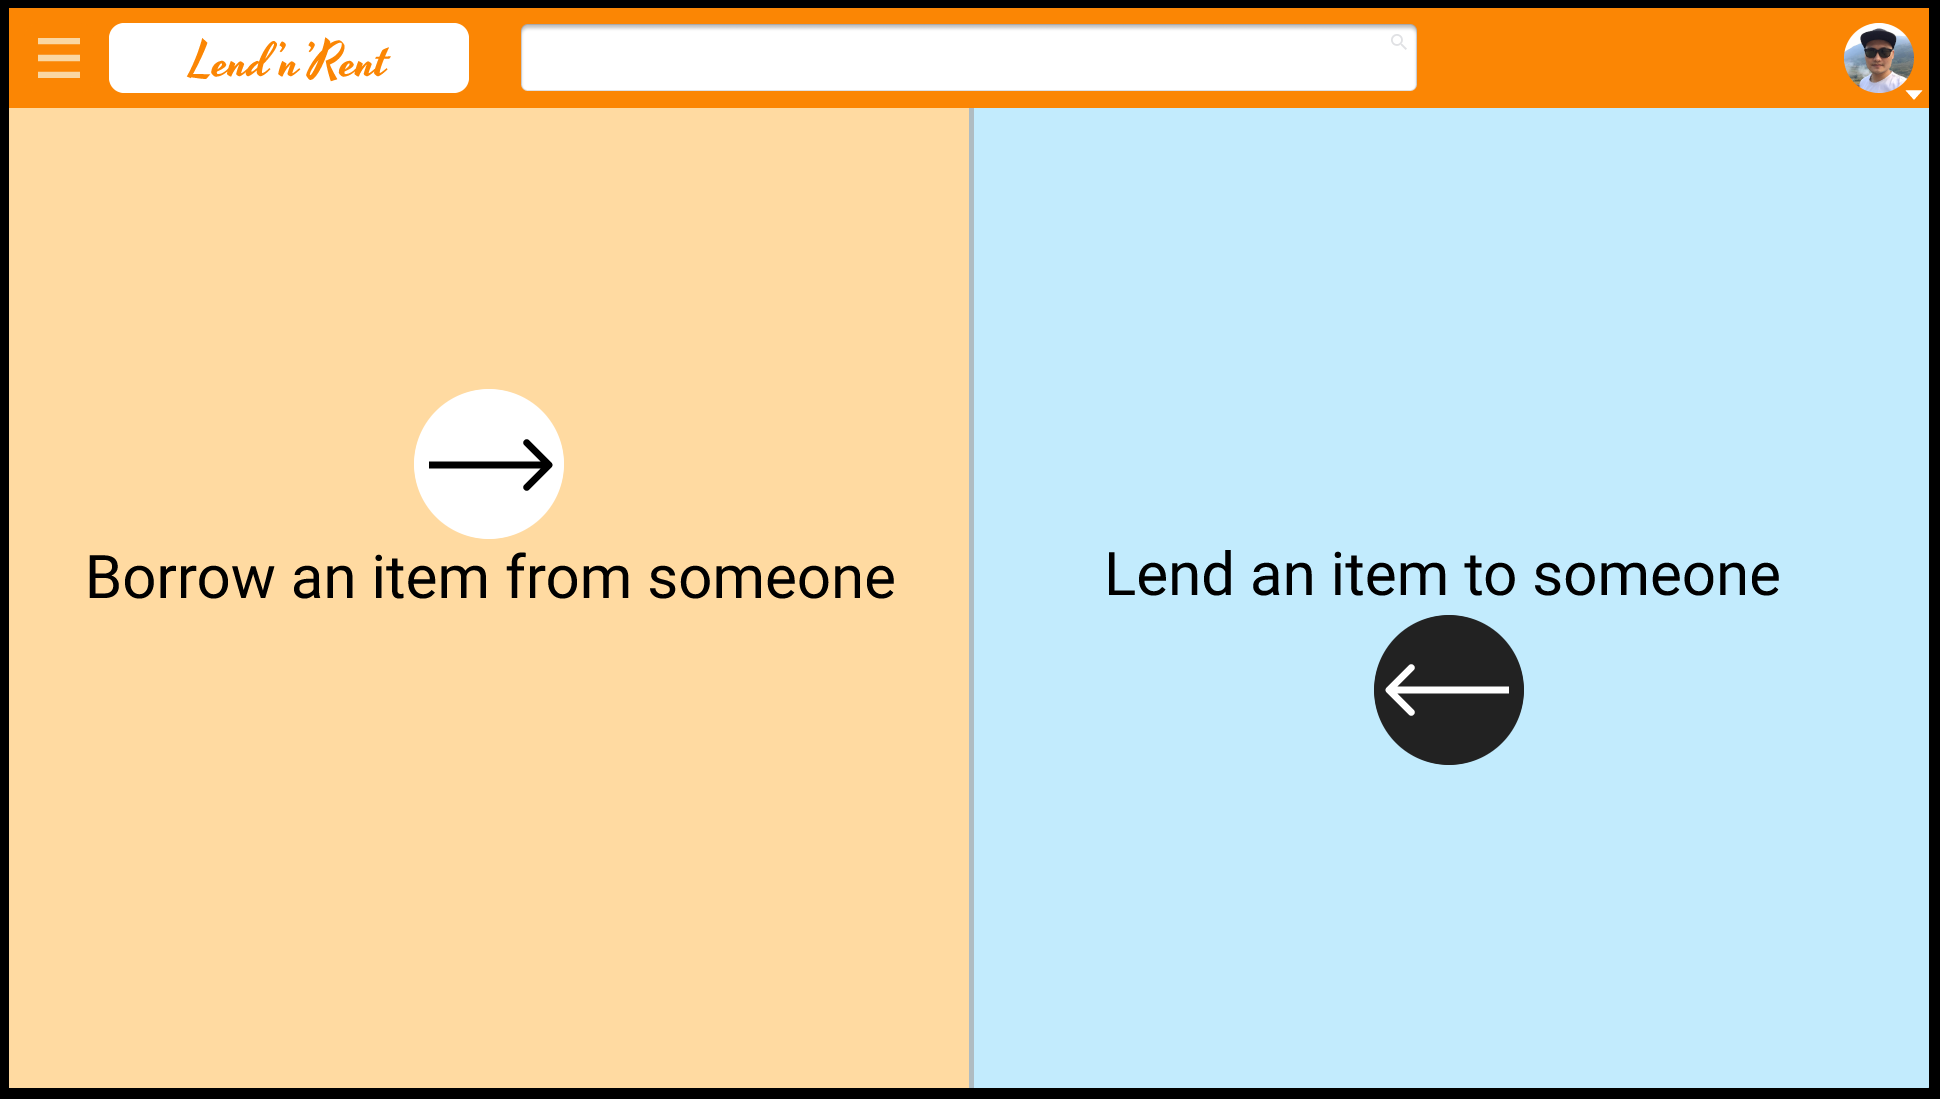
\includegraphics[width=0.5\linewidth]{abb/1landing}
	\caption{Landing page}
	\label{fig:1landing}
\end{figure} 

\noindent
The unique color design of our website makes it always obvious to the user whether he is in the role of lender or renter. If the user rents items, his profile page will also be displayed in the respective blue color scheme, or in orange if he removes all items.

\begin{figure}[H]
	\centering
	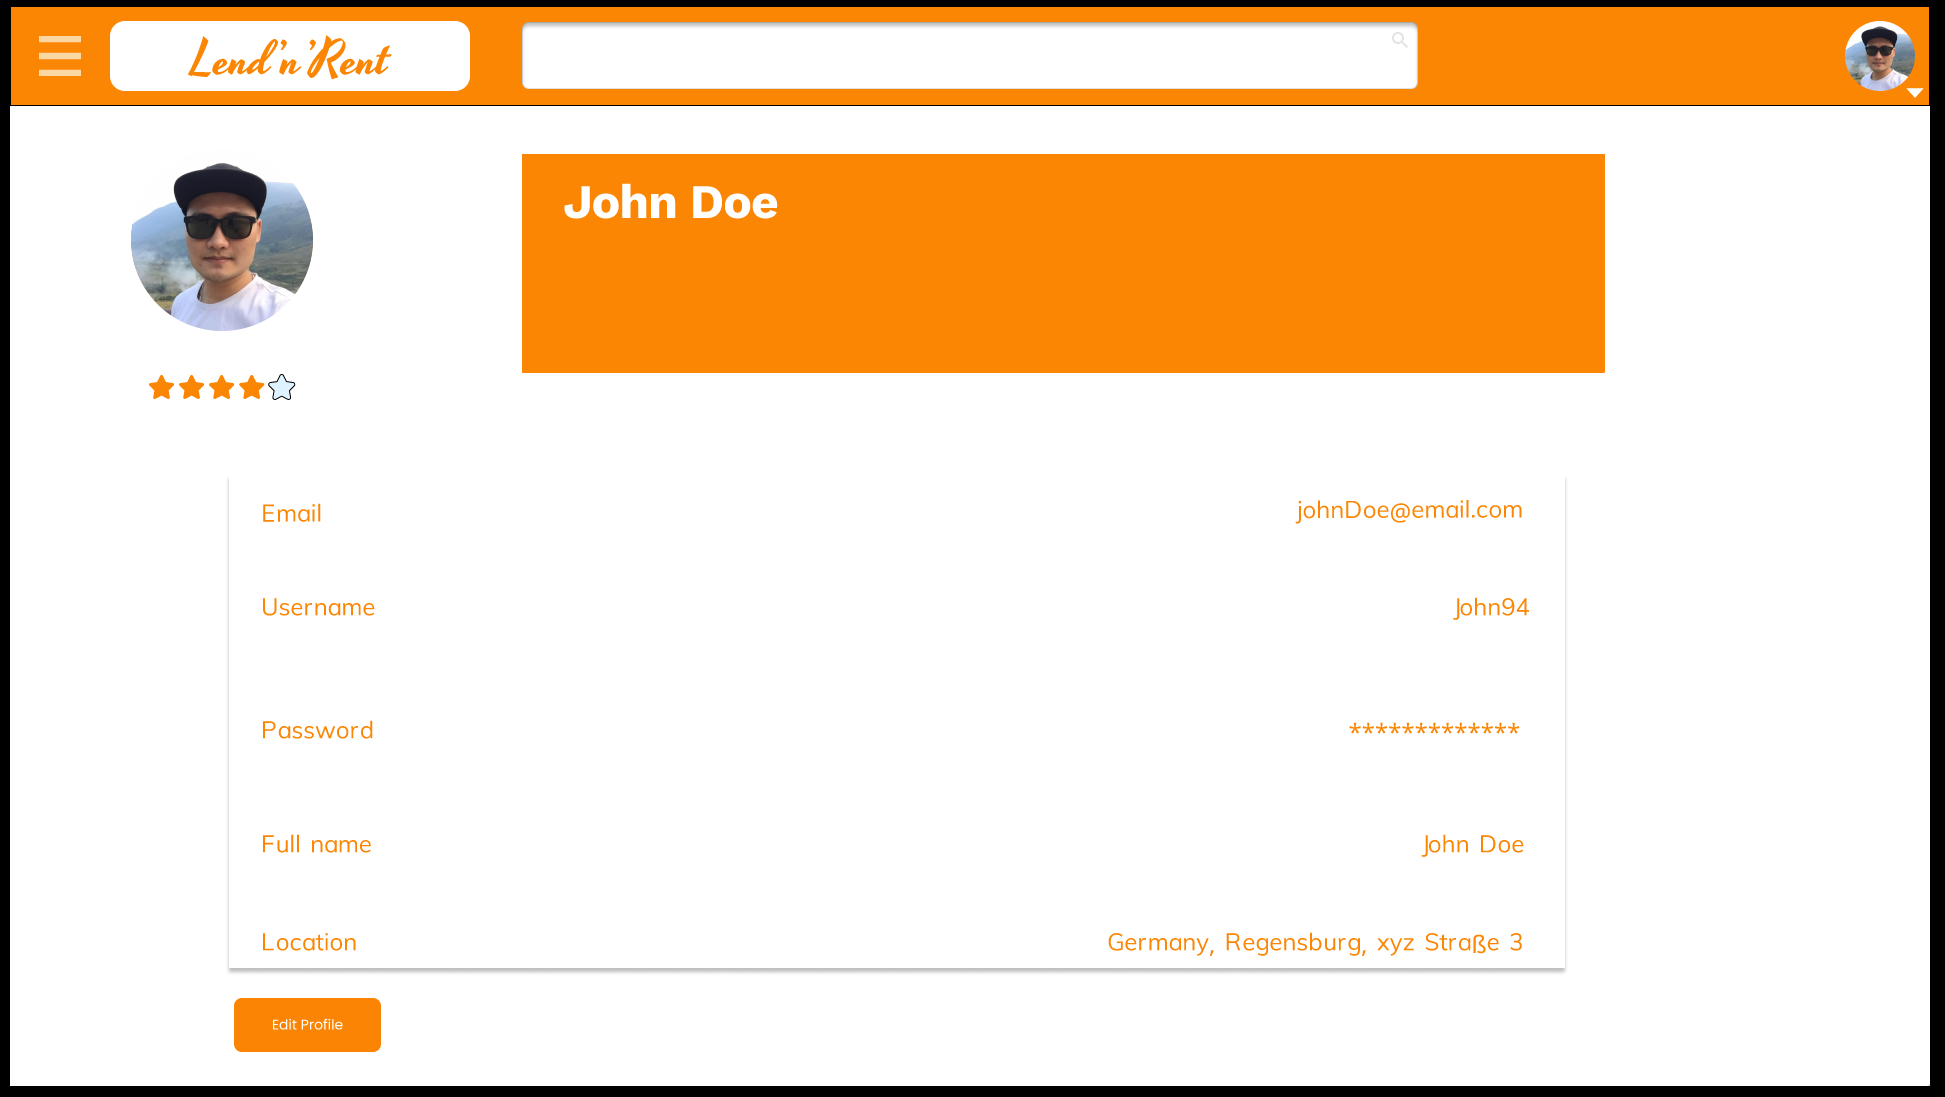
\includegraphics[width=0.49\linewidth]{abb/11profilerent}
	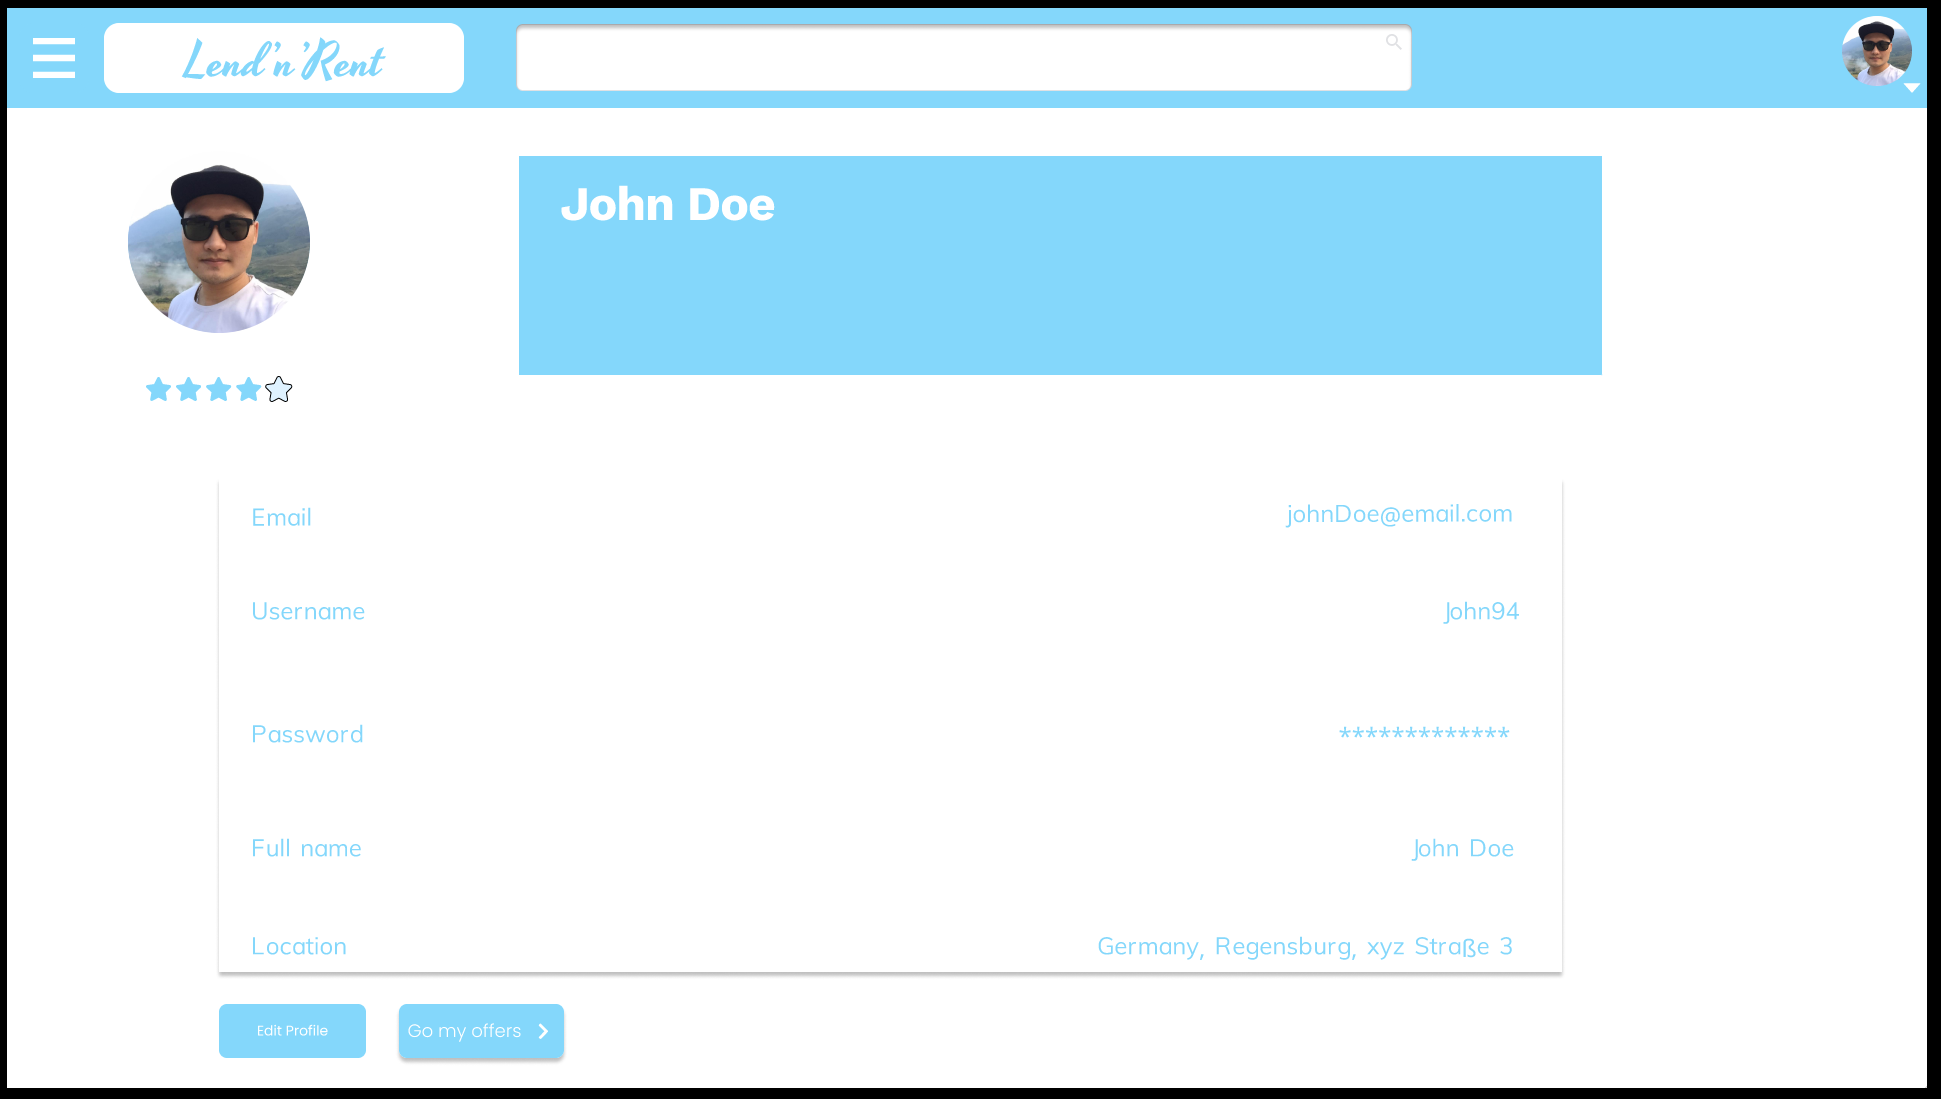
\includegraphics[width=0.49\linewidth]{abb/6profilelend}
	\caption{Profilepage lender and renter}
	\label{fig:profile}
	\centering
\end{figure}

\noindent
The create an offer process is very simple and allows the lender to compare his item with others in order to choose a competitive price.

\begin{figure}[H]
	\centering
	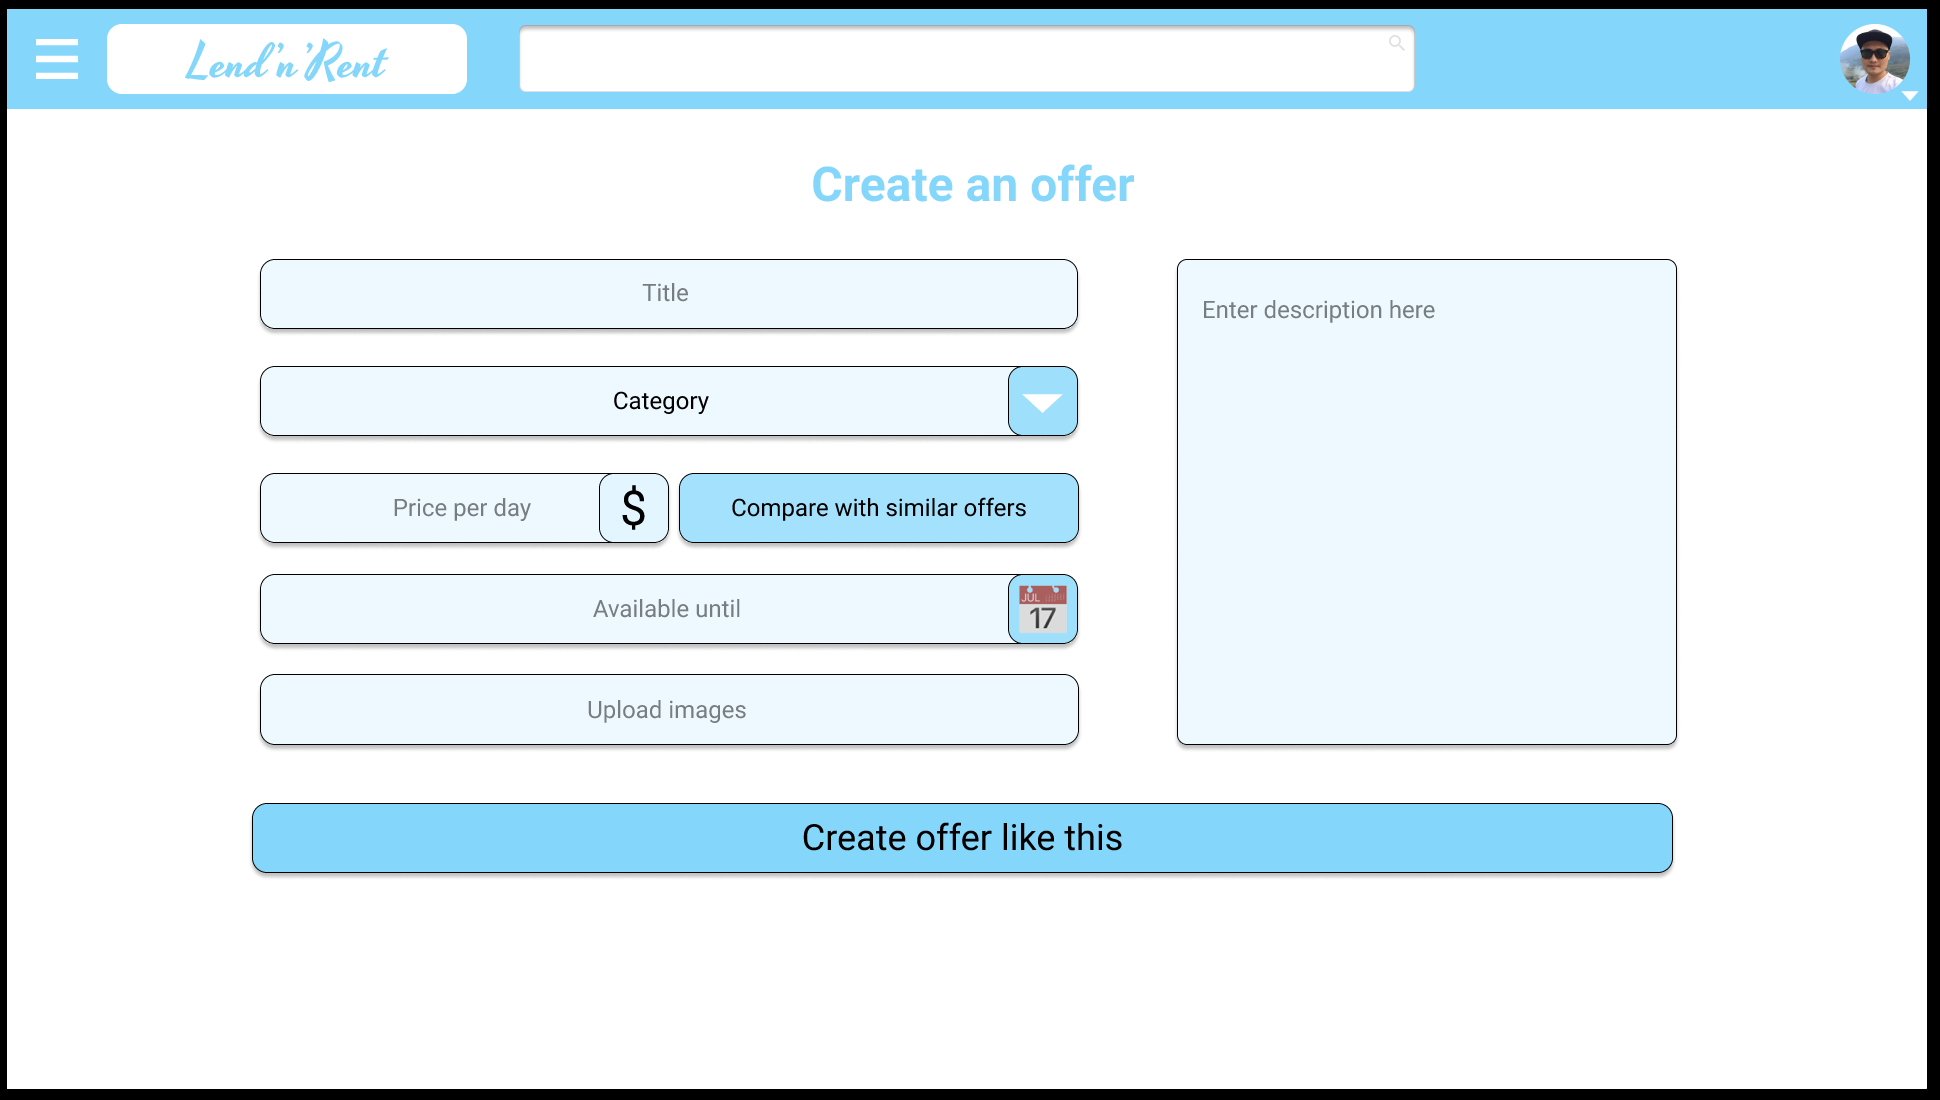
\includegraphics[width=0.5\linewidth]{abb/2offer}
	\caption{Create offer}
	\label{fig:2offer}
\end{figure} 

\noindent
After creating the offer, the user is navigated to the item page to get an overview and make any changes. An overview of all items can be found on the my offers page.

\begin{figure}[H]
	\centering
	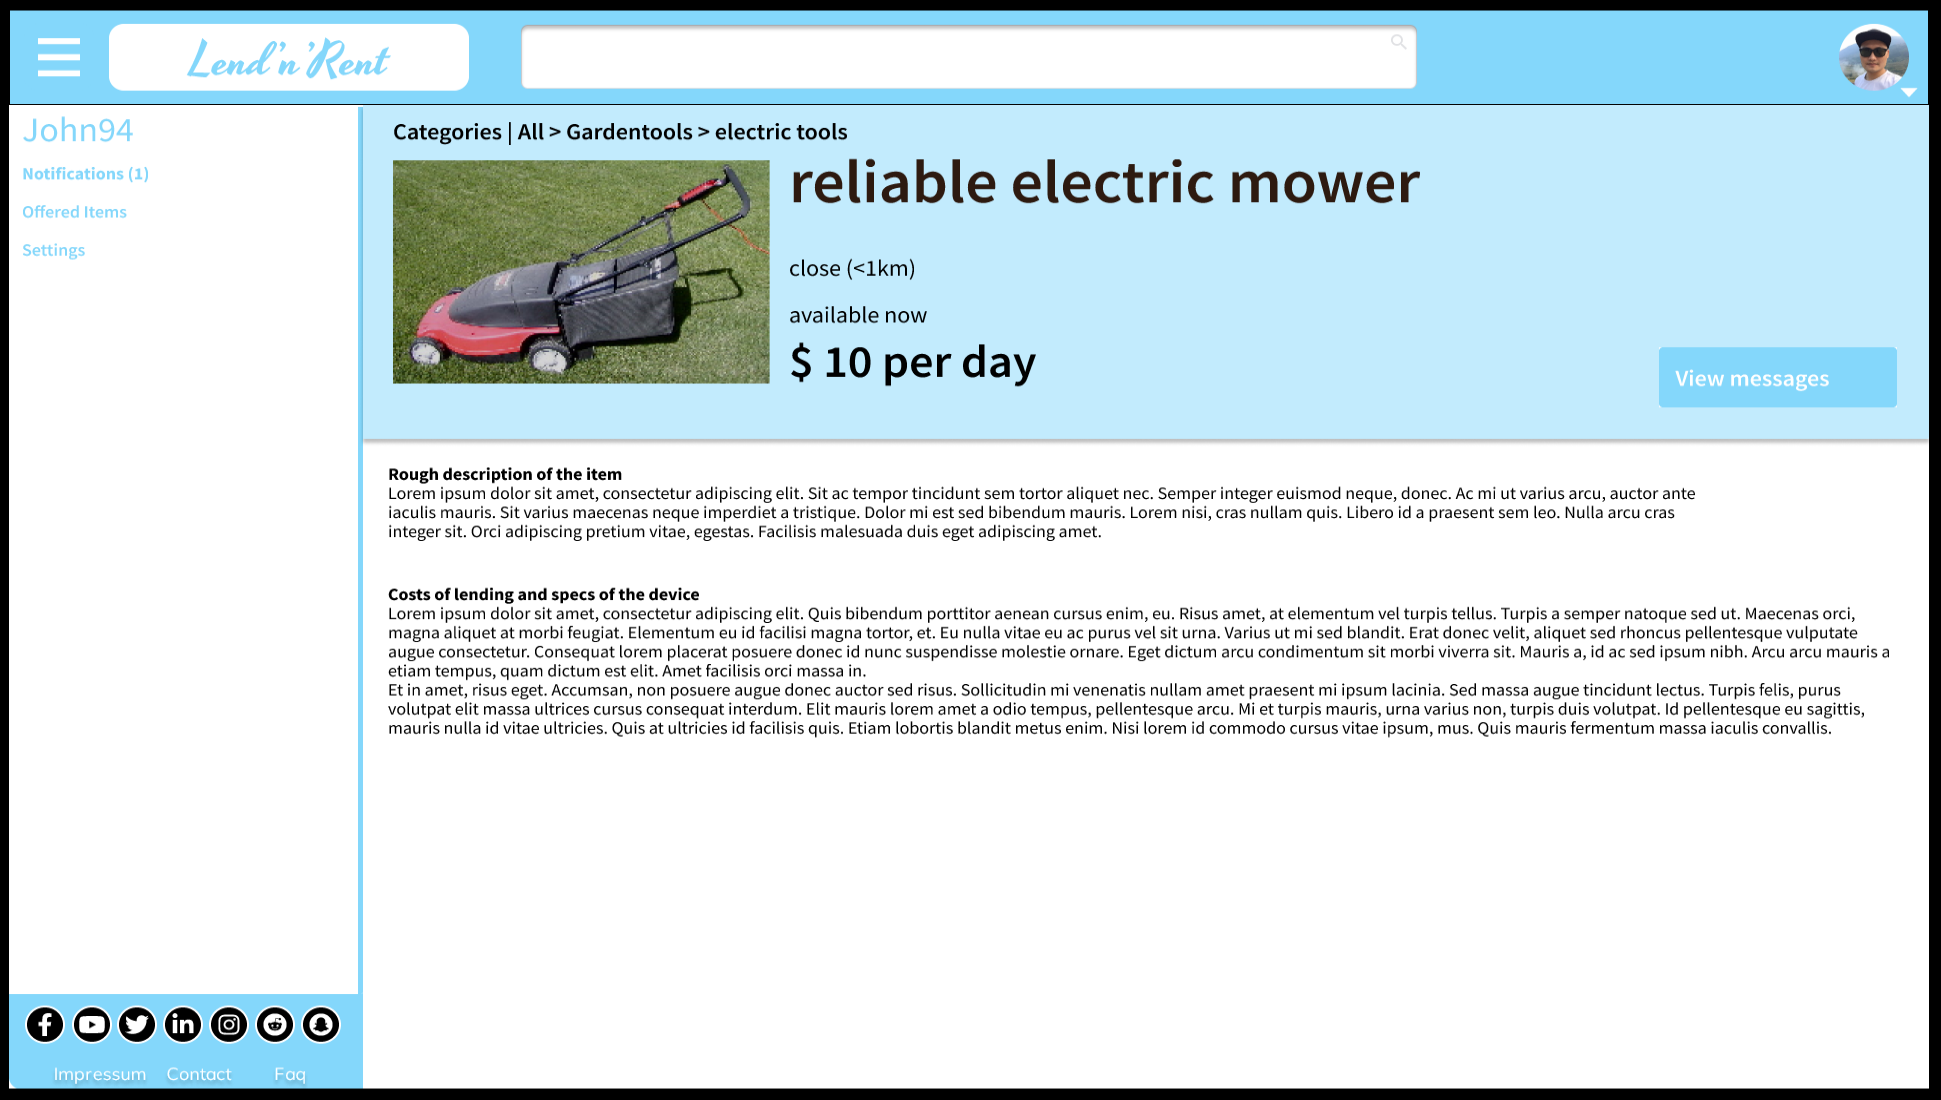
\includegraphics[width=0.49\linewidth]{abb/4item}
	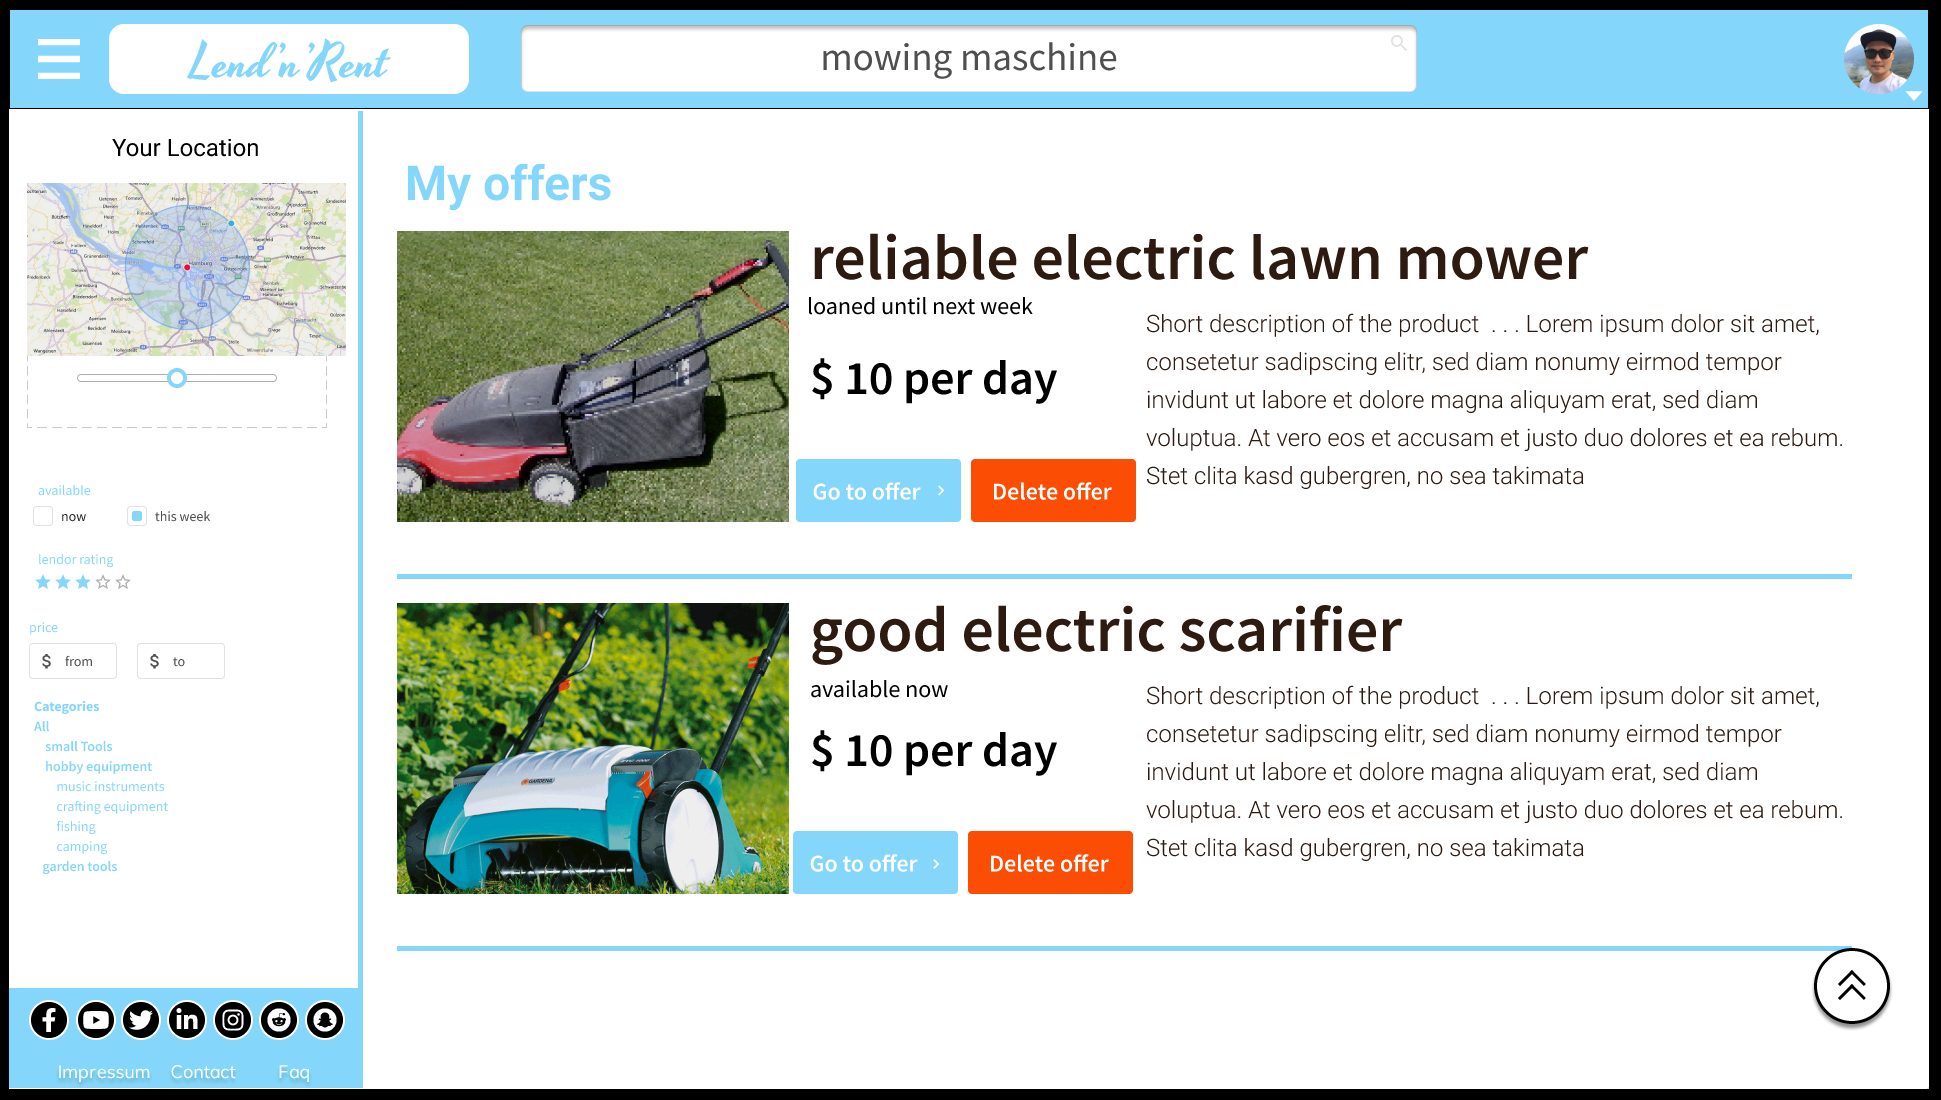
\includegraphics[width=0.49\linewidth]{abb/3offers}
	\caption{Article and offers page}
	\label{fig:article}
	\centering
\end{figure}

\noindent
The category page is designed so that the individual categories are displayed as large images. The idea behind this is not to flood the user with a lot of information, but to leave it up to the user to make a concrete decision.

\begin{figure}[H]
	\centering
	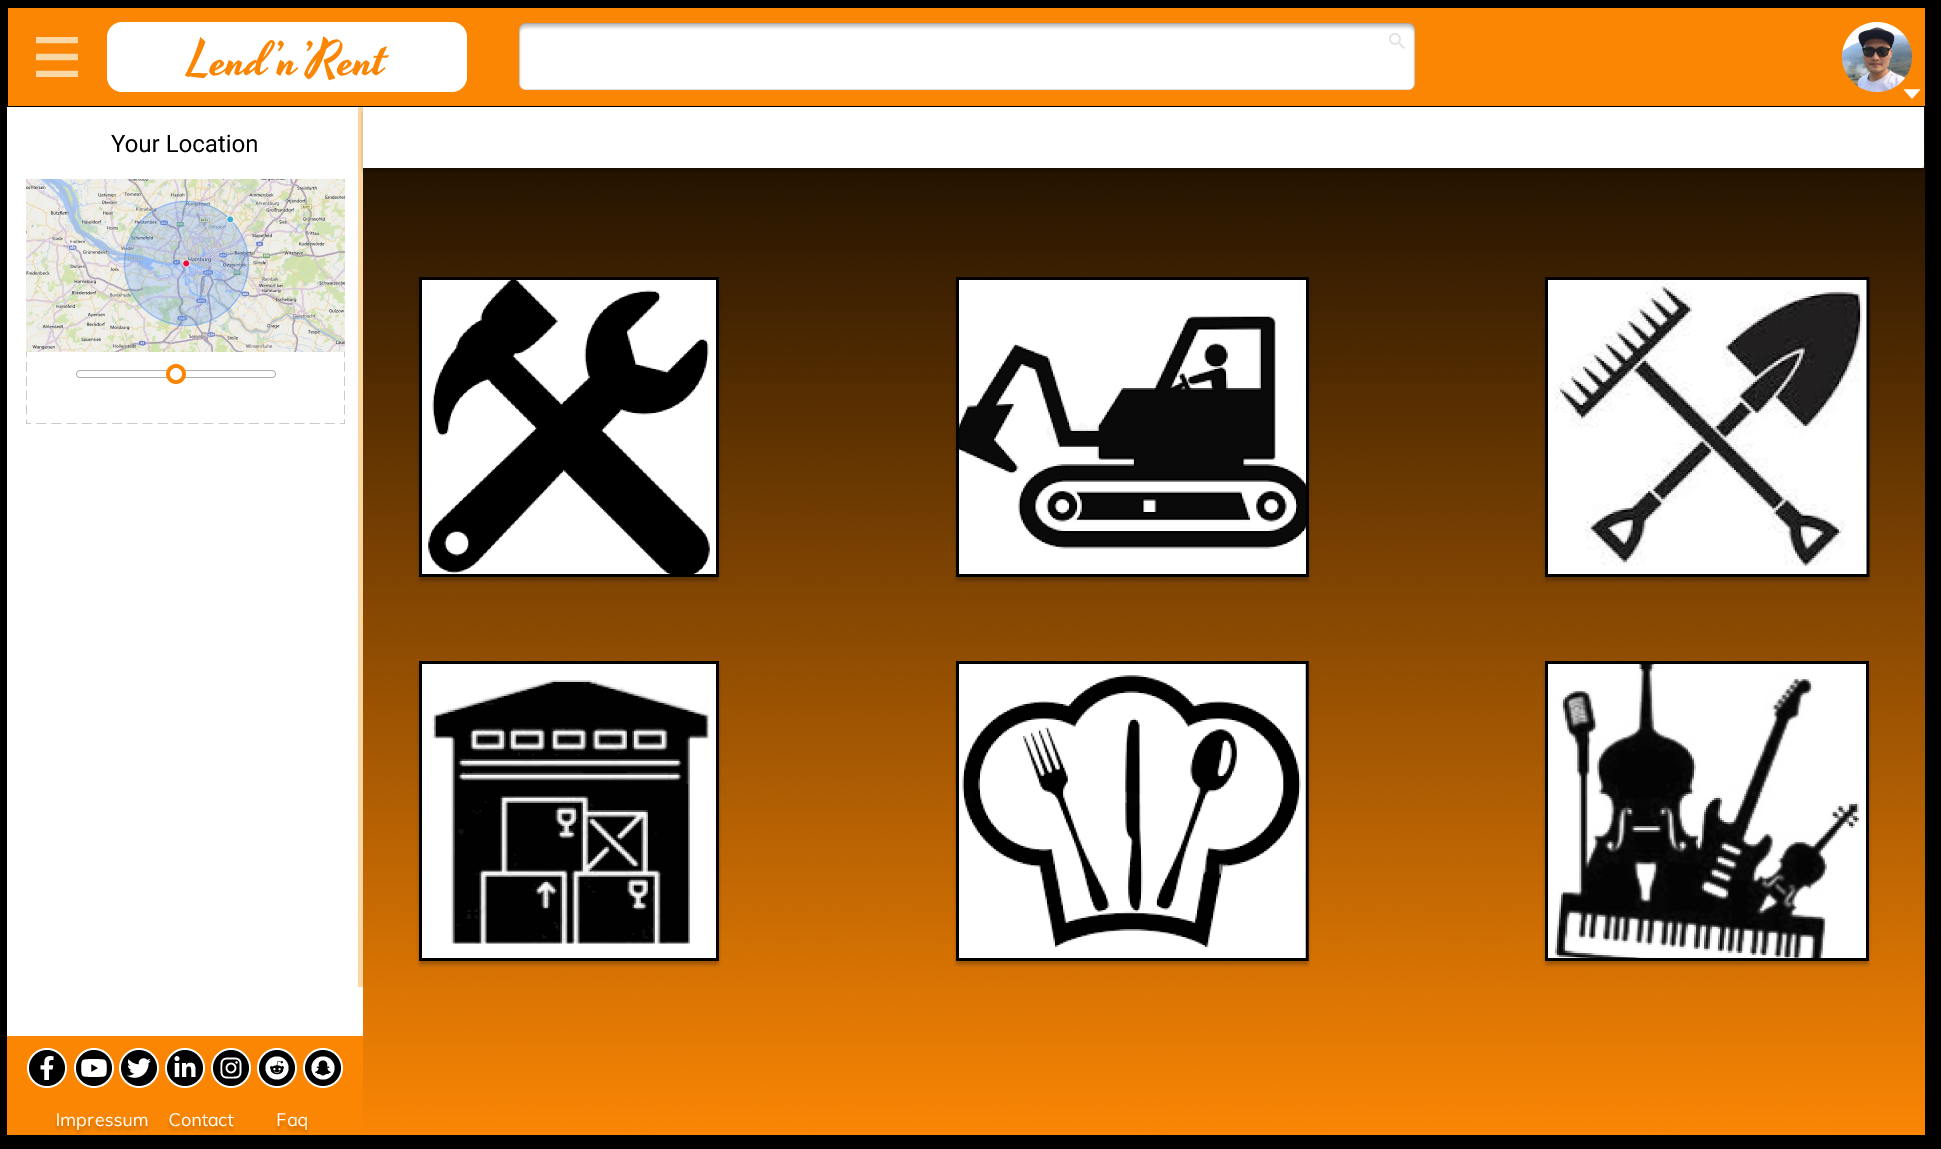
\includegraphics[width=0.5\linewidth]{abb/8start}
	\caption{Category page}
	\label{fig:8start}
\end{figure} 

\noindent
Only after the user has chosen a category, he will be redirected to the search page and the items from this category will be displayed.
On the search page the user has the possibility to choose a subcategory, set the search radius, price range, availability and average rating.

\begin{figure}[H]
	\centering
	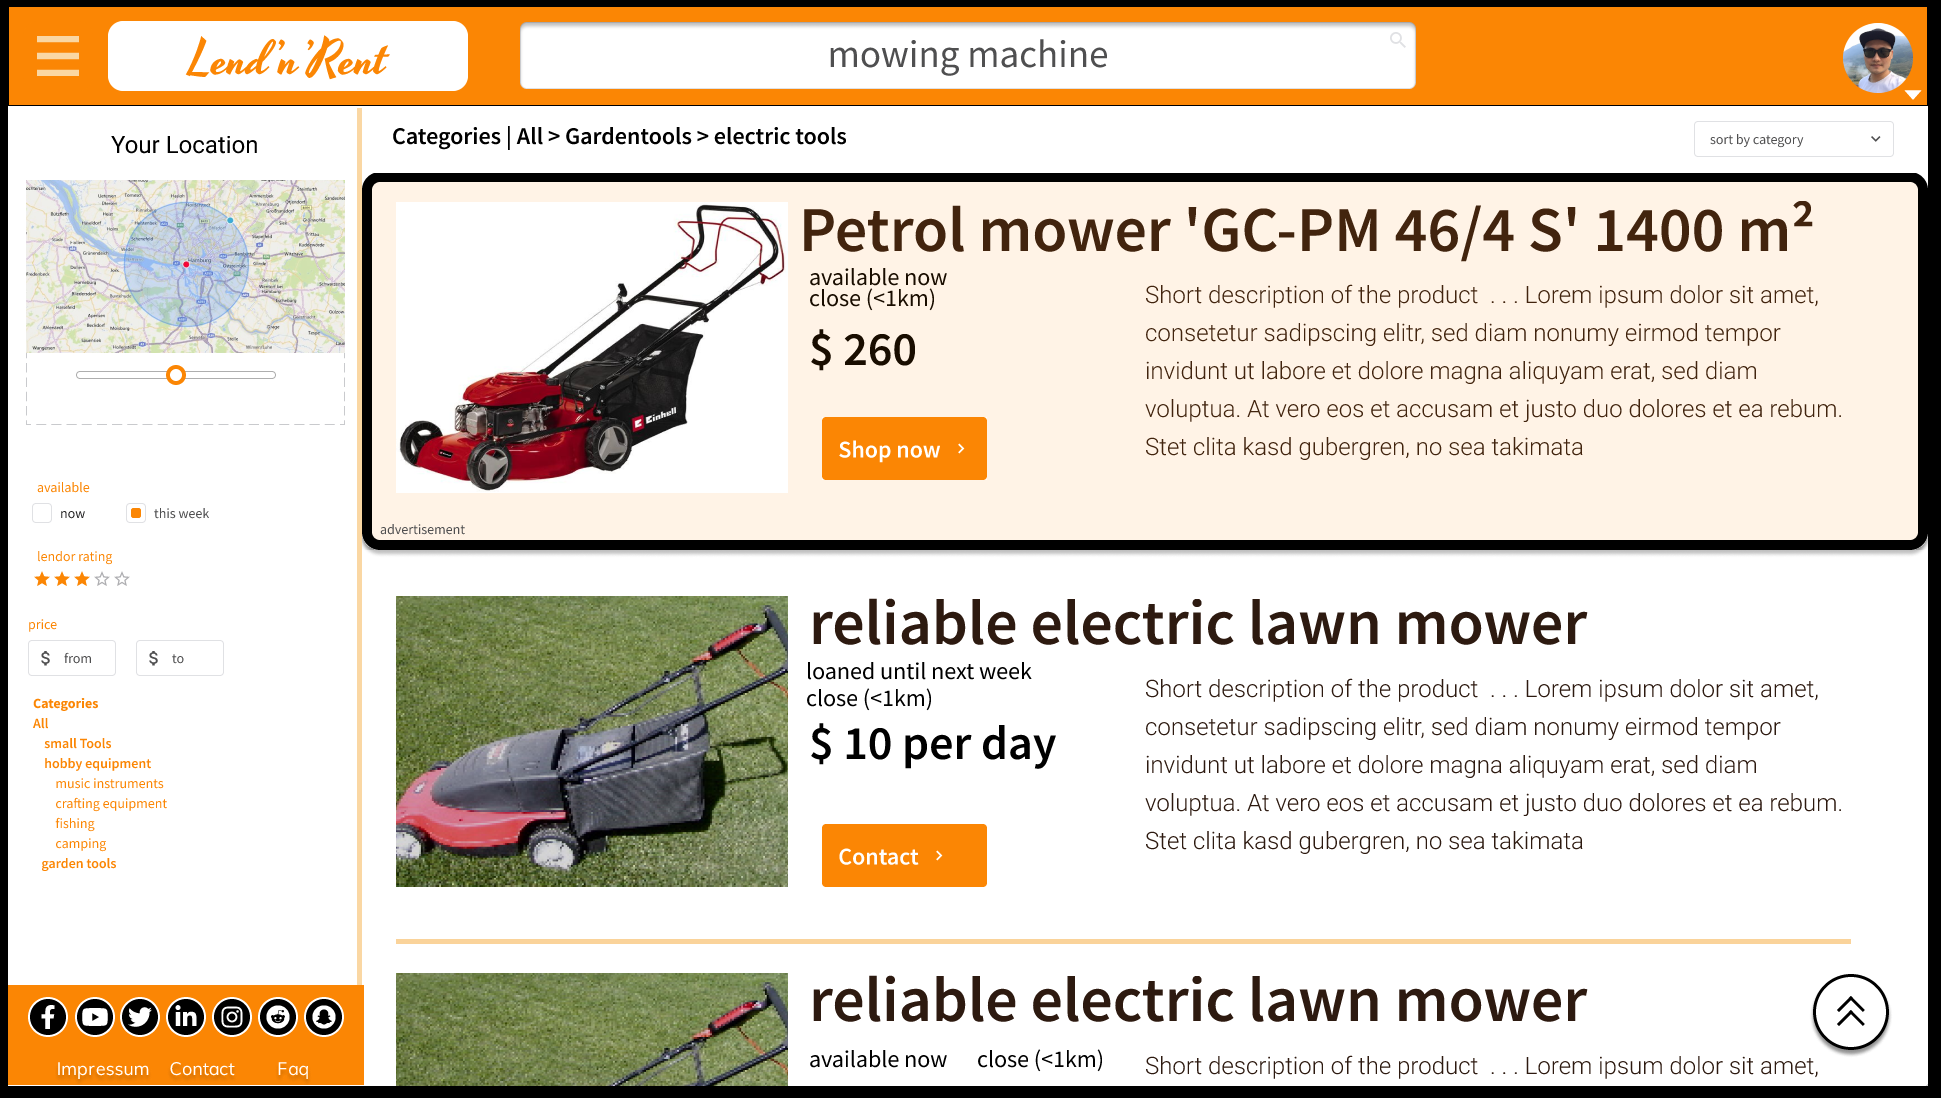
\includegraphics[width=0.49\linewidth]{abb/9search}
	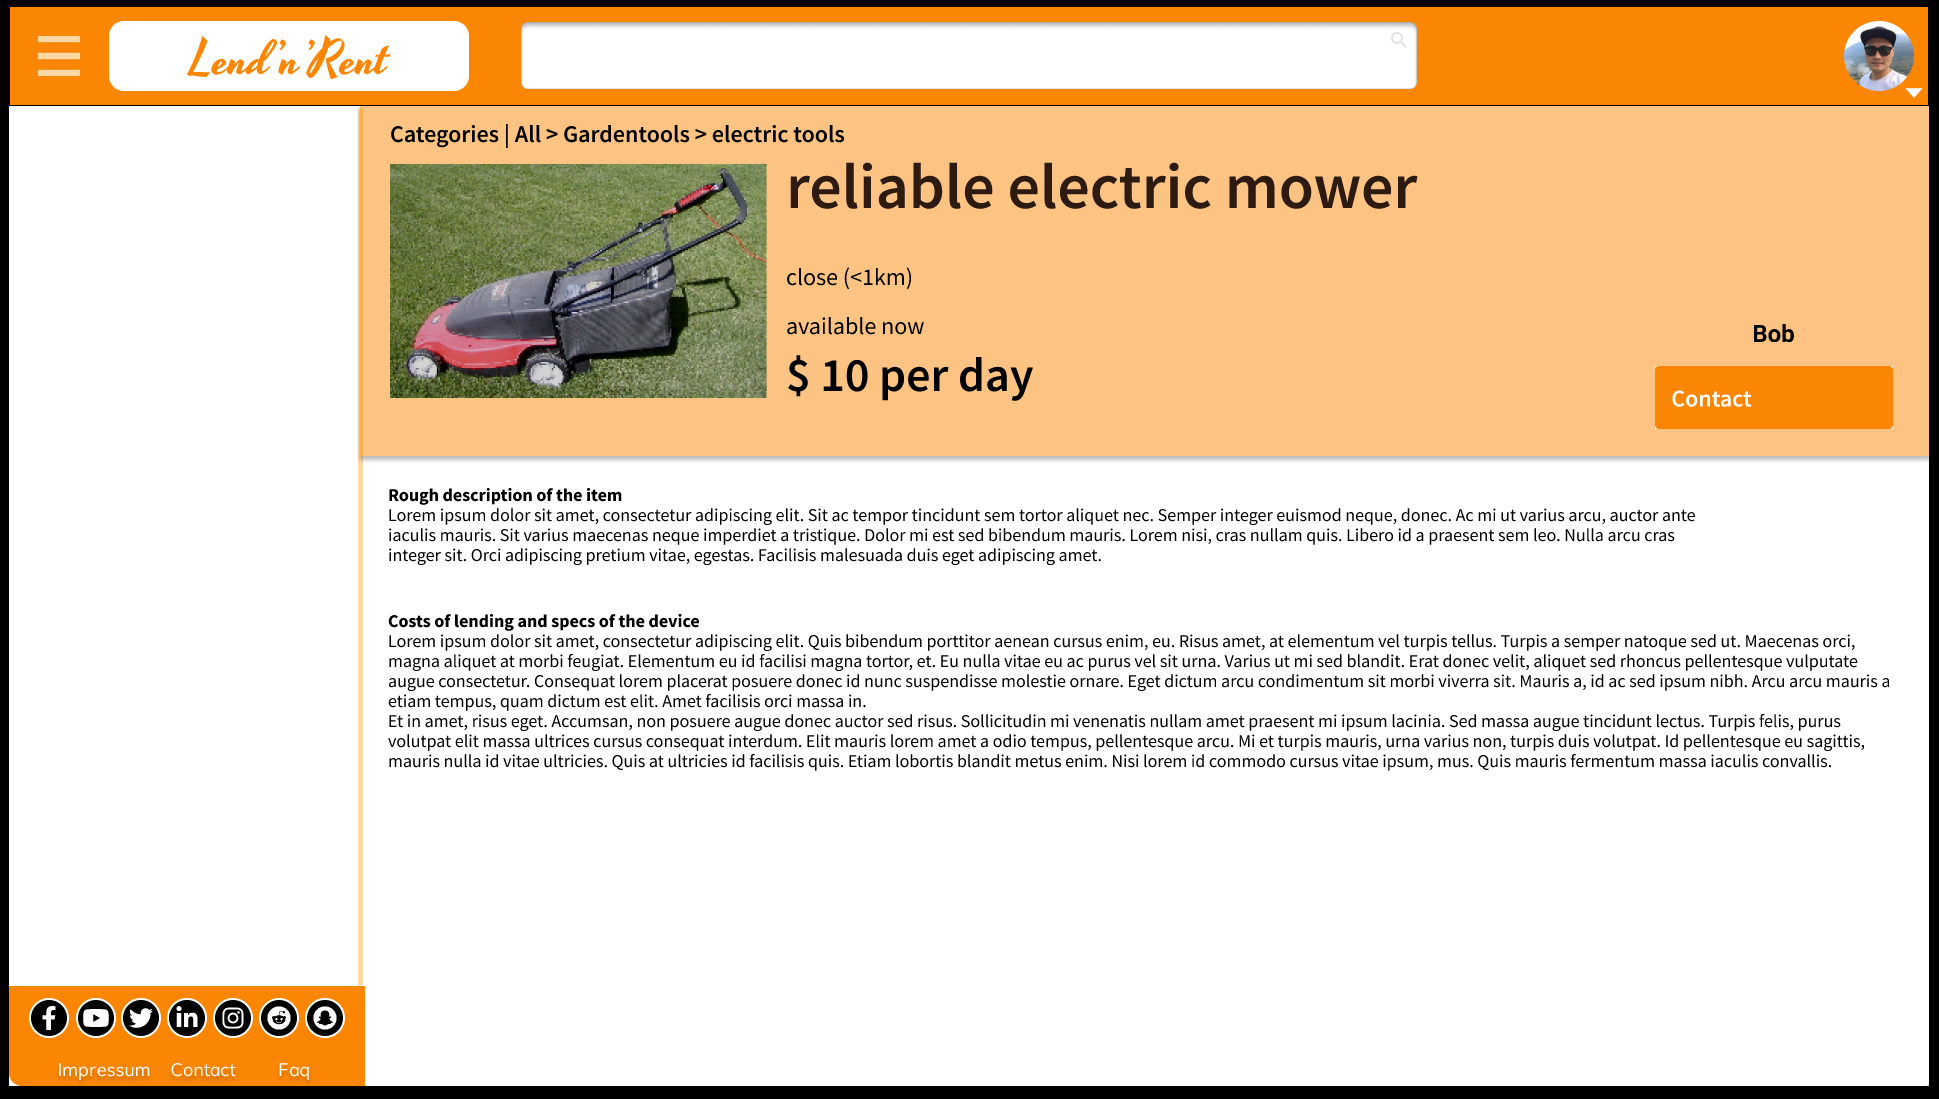
\includegraphics[width=0.49\linewidth]{abb/10itemrent}
	\caption{Search and article page renter role}
	\label{fig:search}
	\centering
\end{figure}

\newpage
\noindent
As soon as the user has chosen an item, he has the possibility to contact the lender via the article page.

\begin{figure}[H]
	\centering
	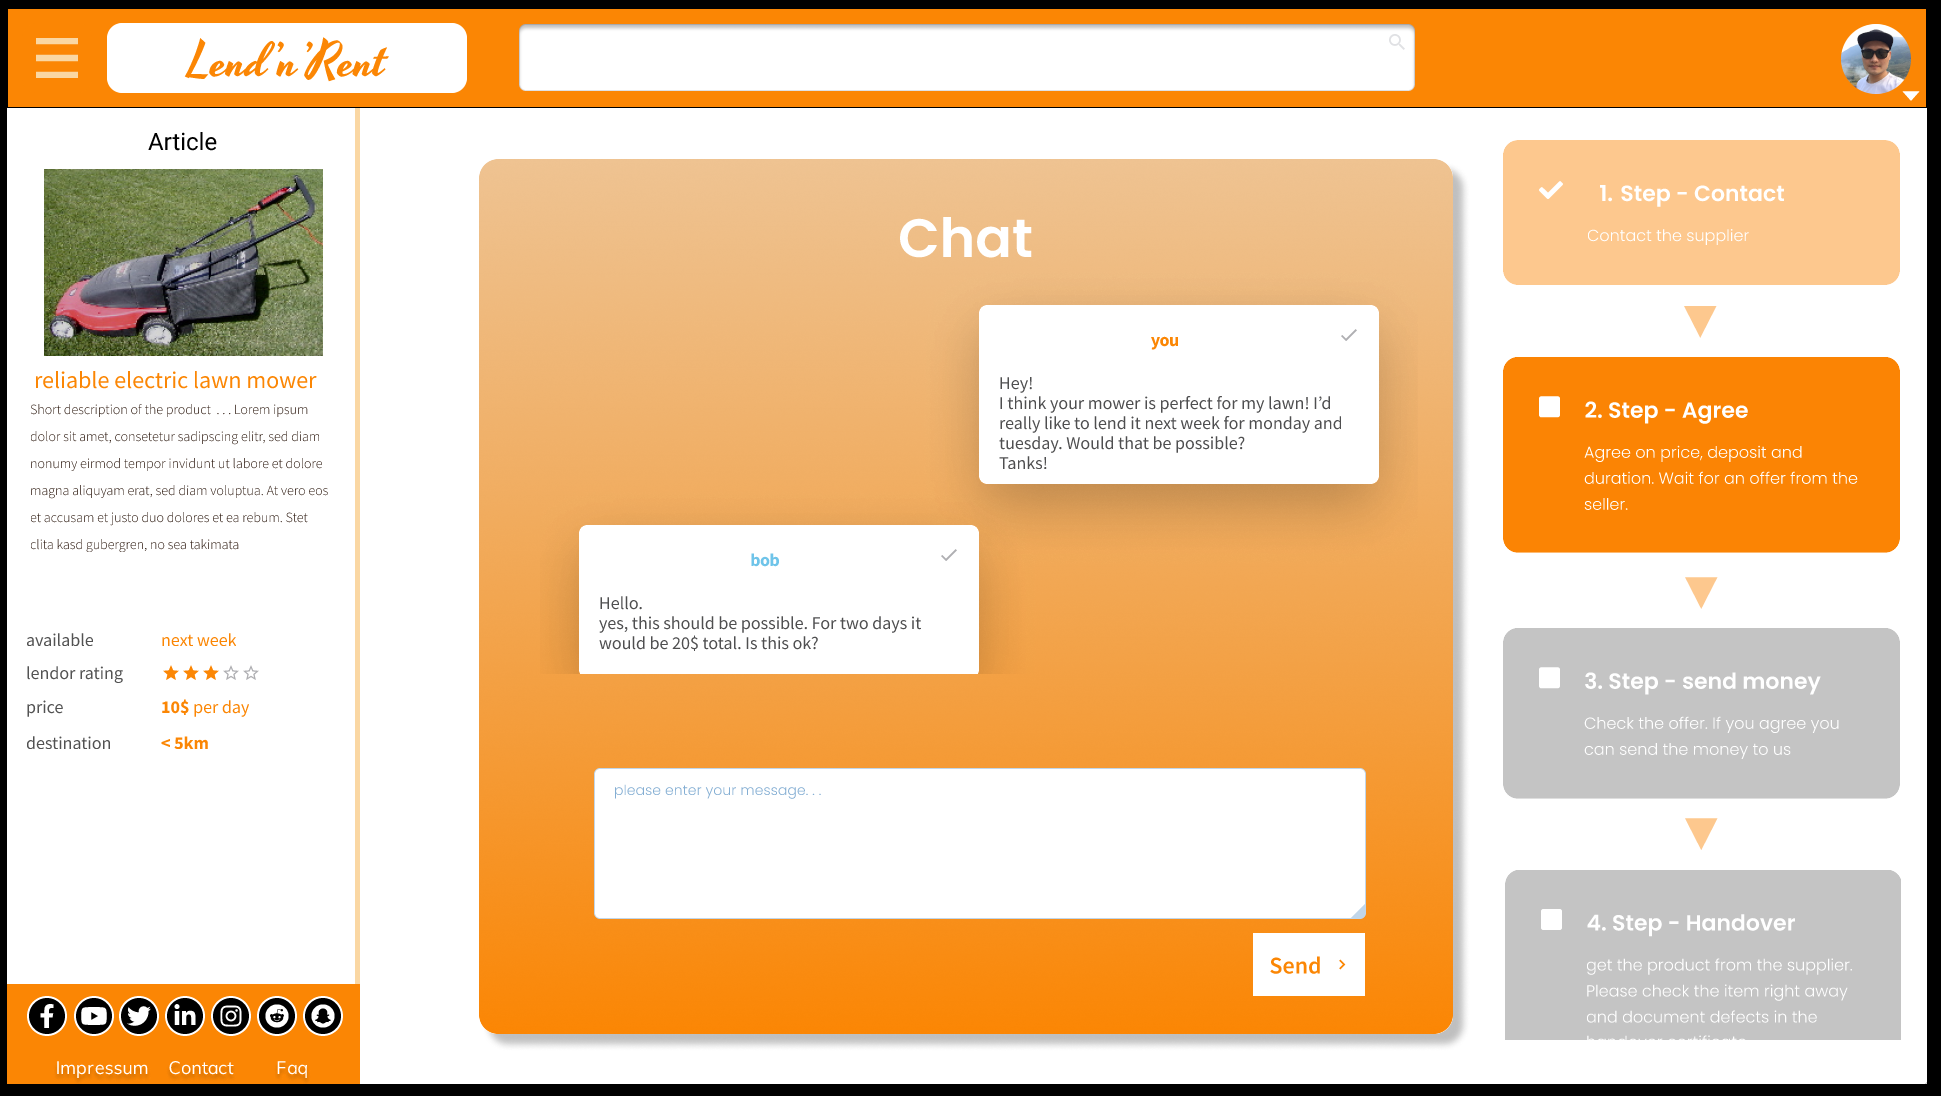
\includegraphics[width=0.49\linewidth]{abb/12step2}
	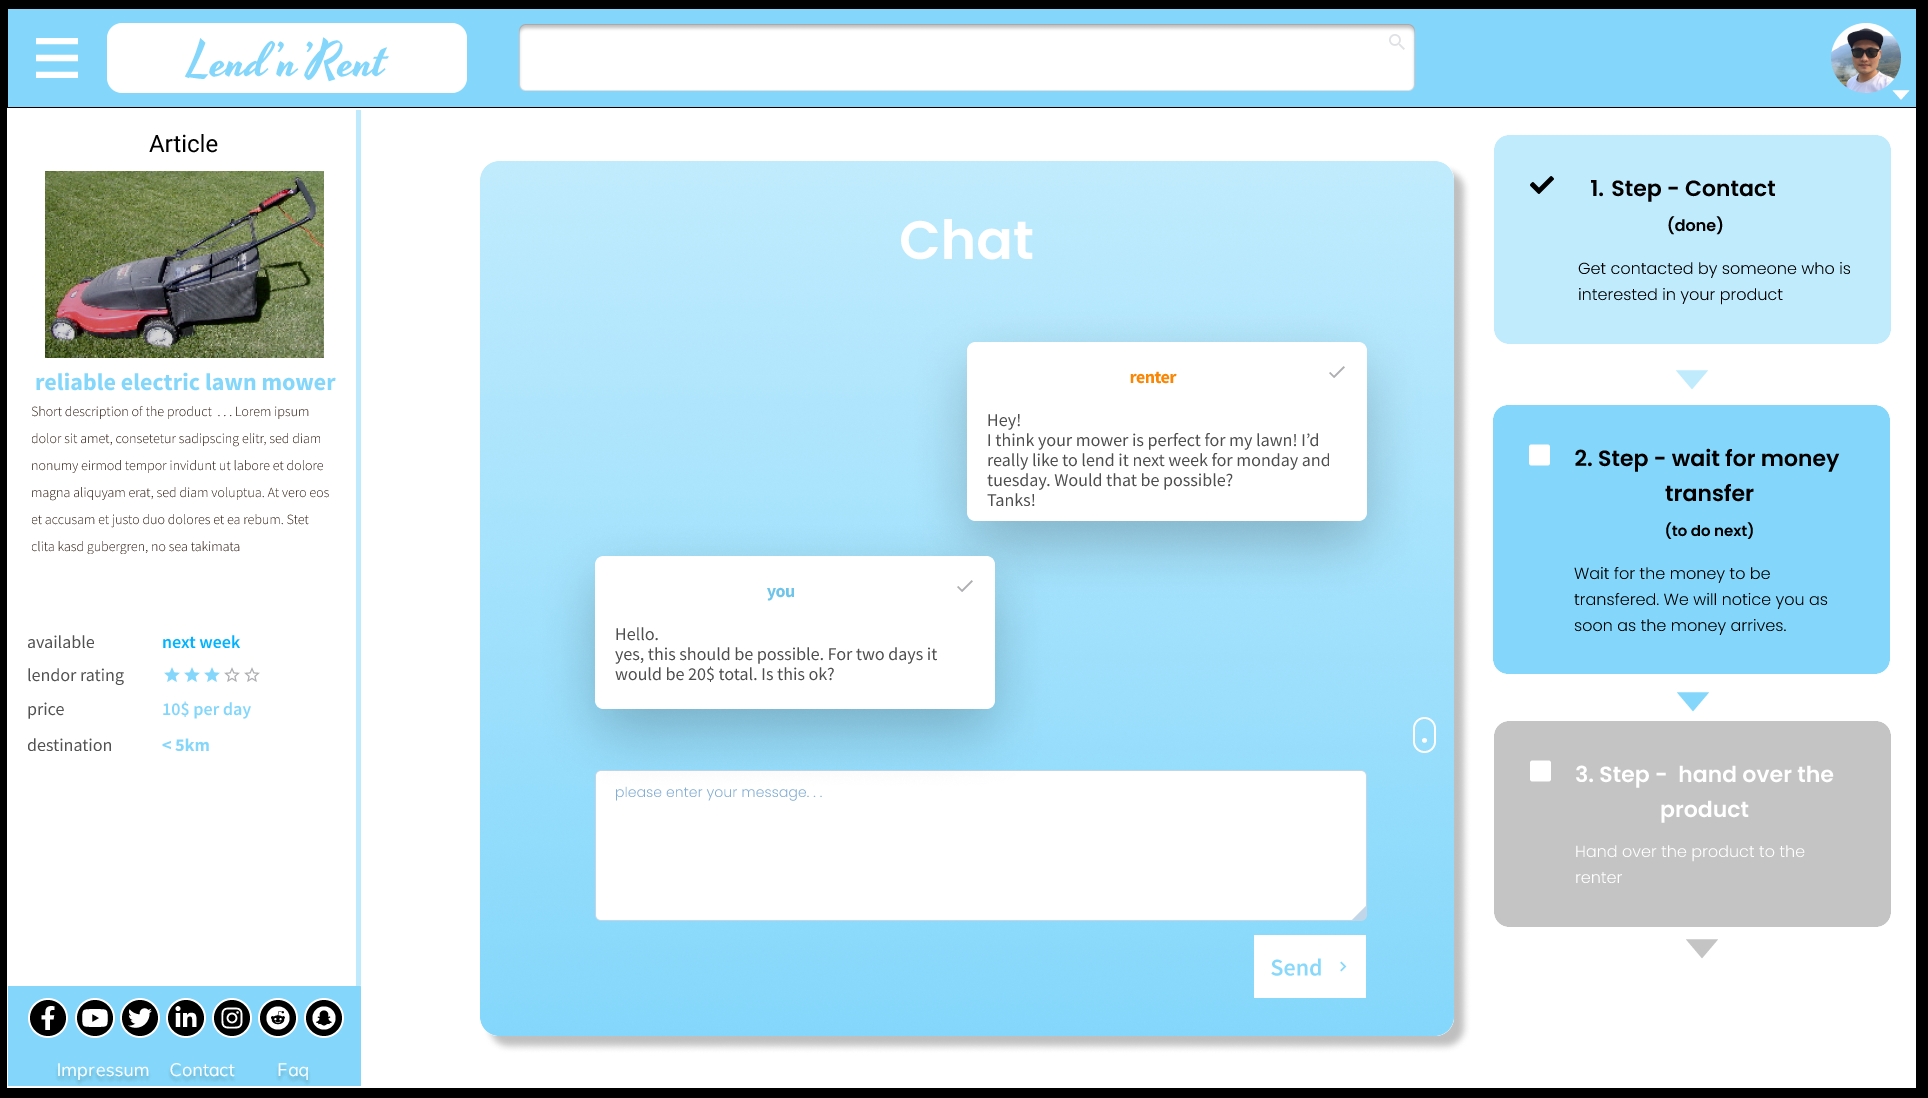
\includegraphics[width=0.49\linewidth]{abb/5step1}
	\caption{Negotiation Step 1 Contact and Agreement}
	\label{fig:negotiation1}
	\centering
\end{figure}

\noindent
Once the users have agreed, the renter must fill in and confirm the offer form.

\begin{figure}[H]
	\centering
	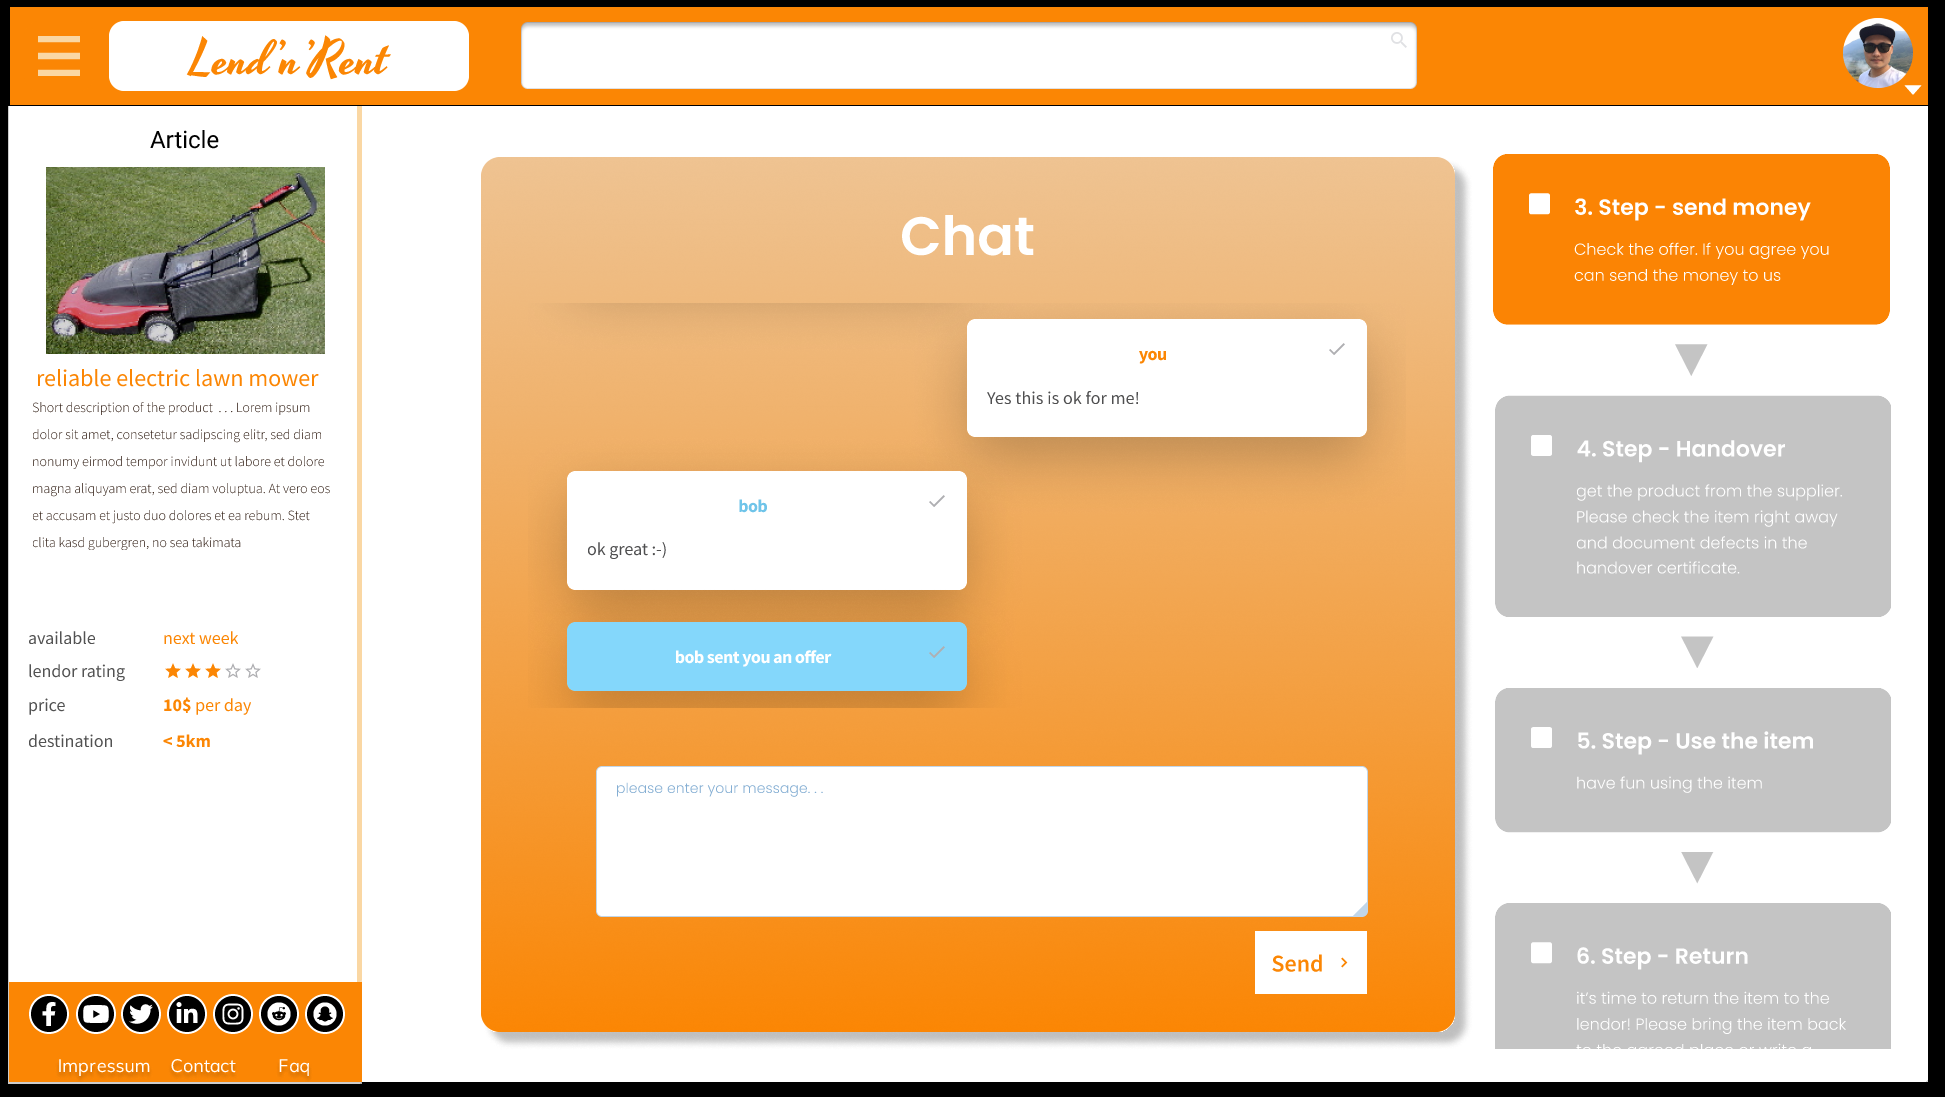
\includegraphics[width=0.49\linewidth]{abb/13step3}
	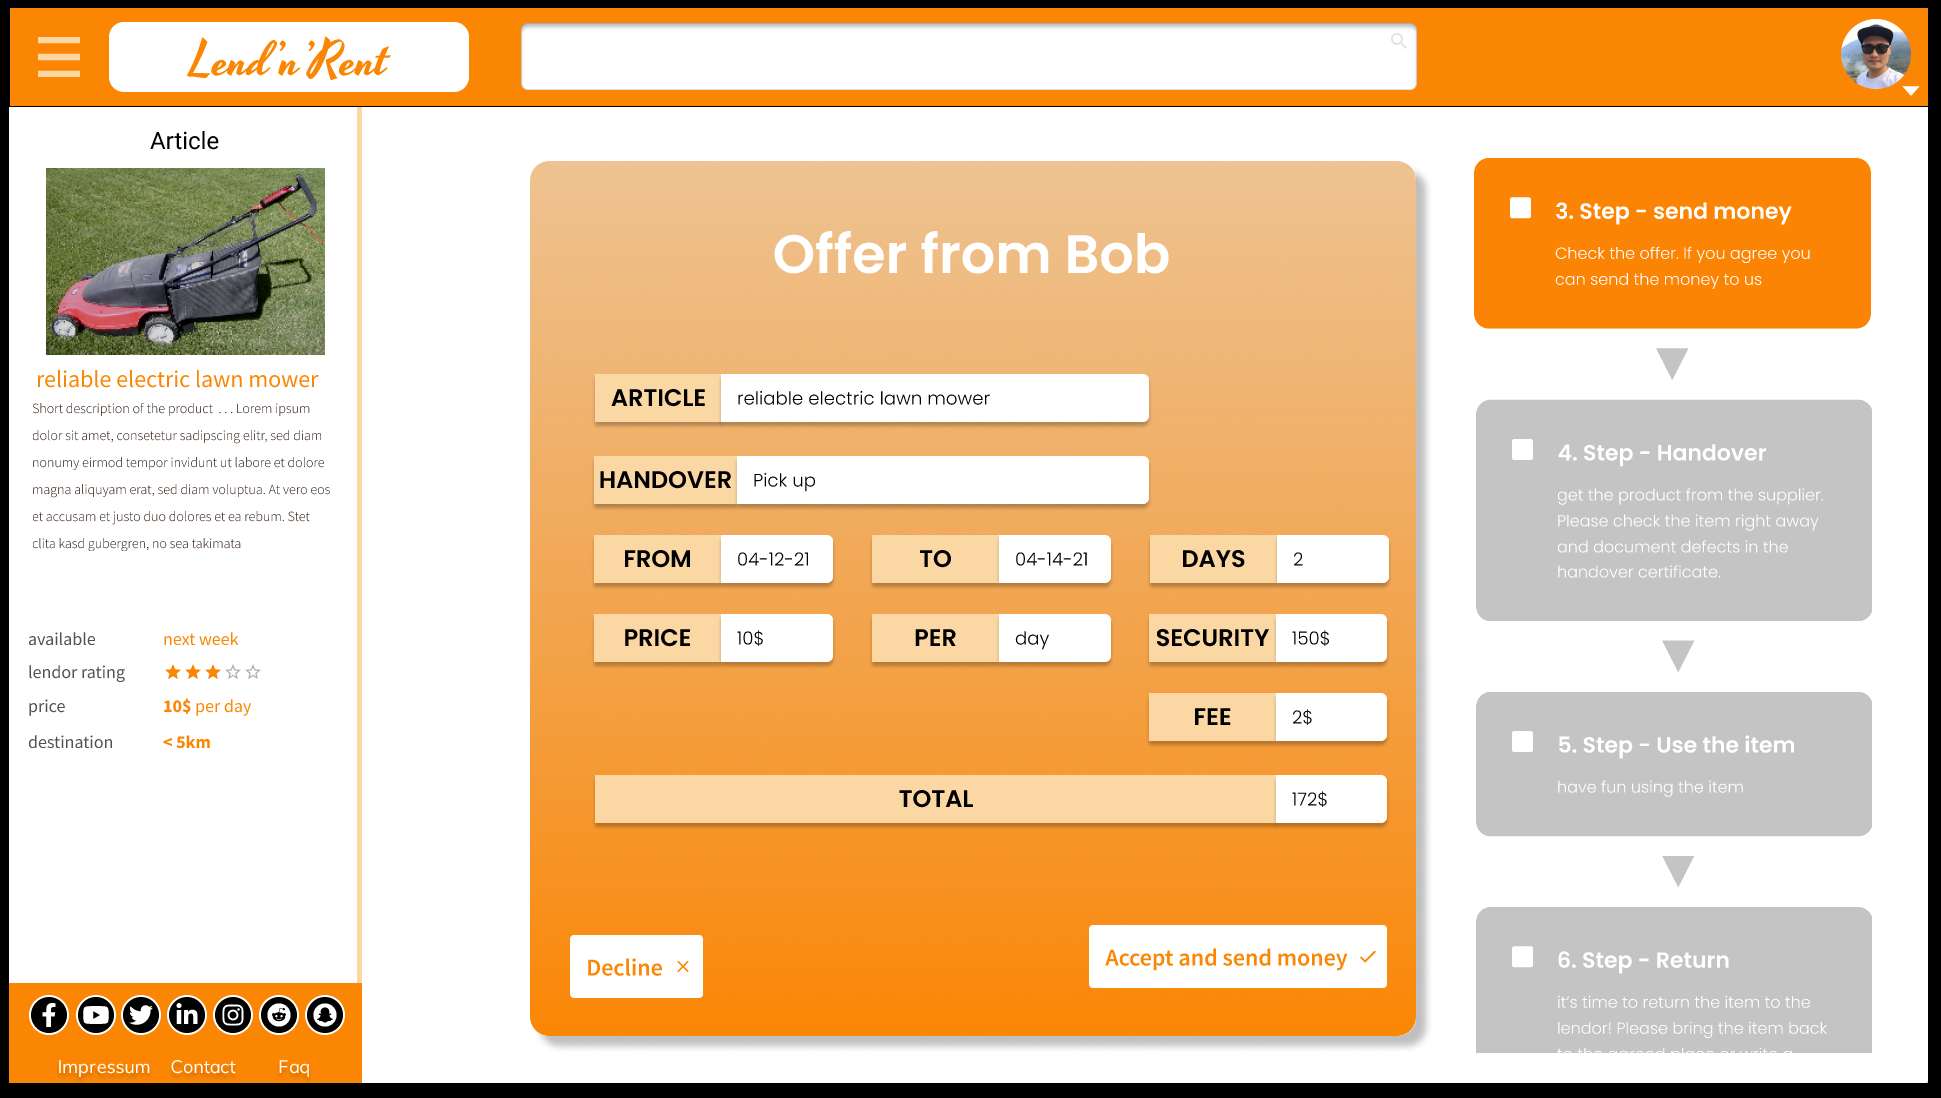
\includegraphics[width=0.49\linewidth]{abb/14step3con}
	\caption{Negotiation Step 3 Payment agreements}
	\label{fig:Negotiation2}
	\centering
\end{figure}

\noindent
After the handover, the renter must inspect the item and describe its condition in the "Handover Certificate" and send the certificate.

\begin{figure}[H]
	\centering
	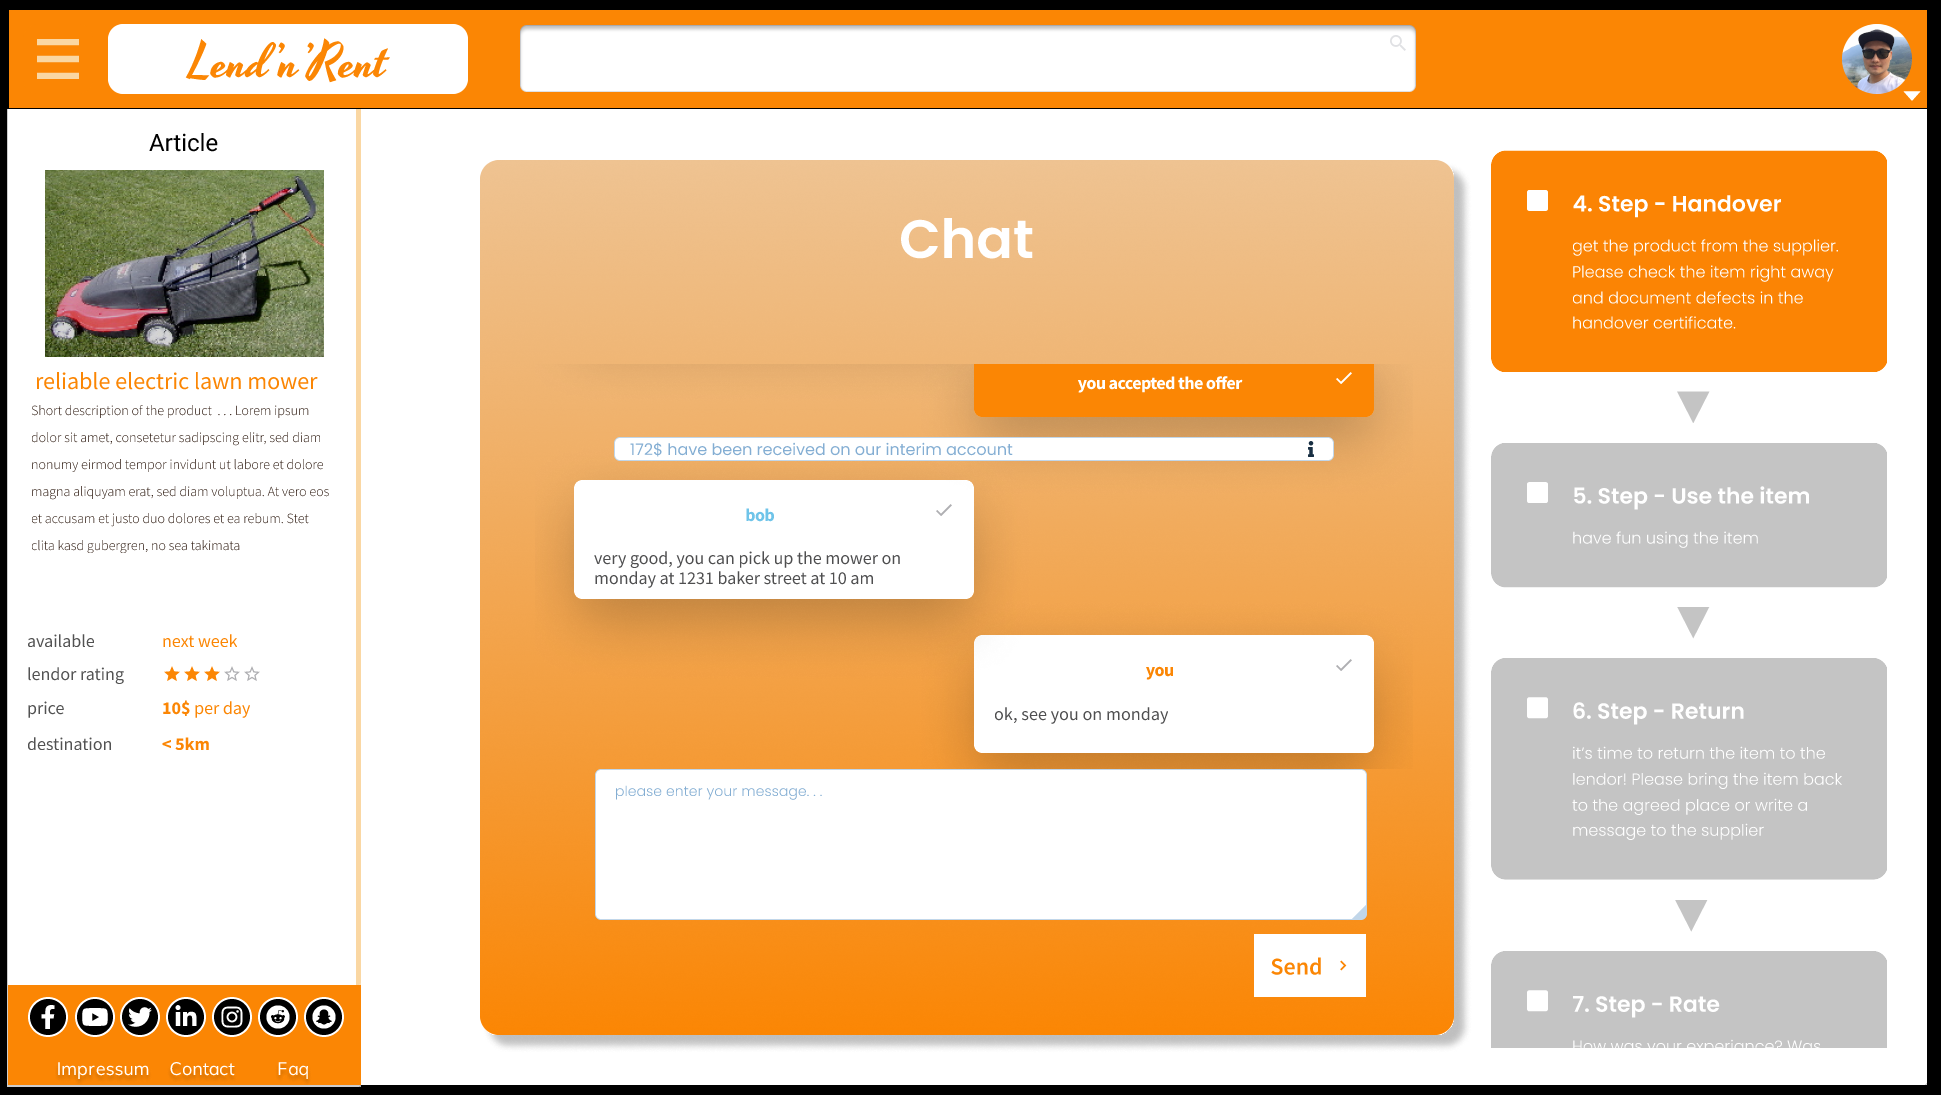
\includegraphics[width=0.49\linewidth]{abb/15step4}
	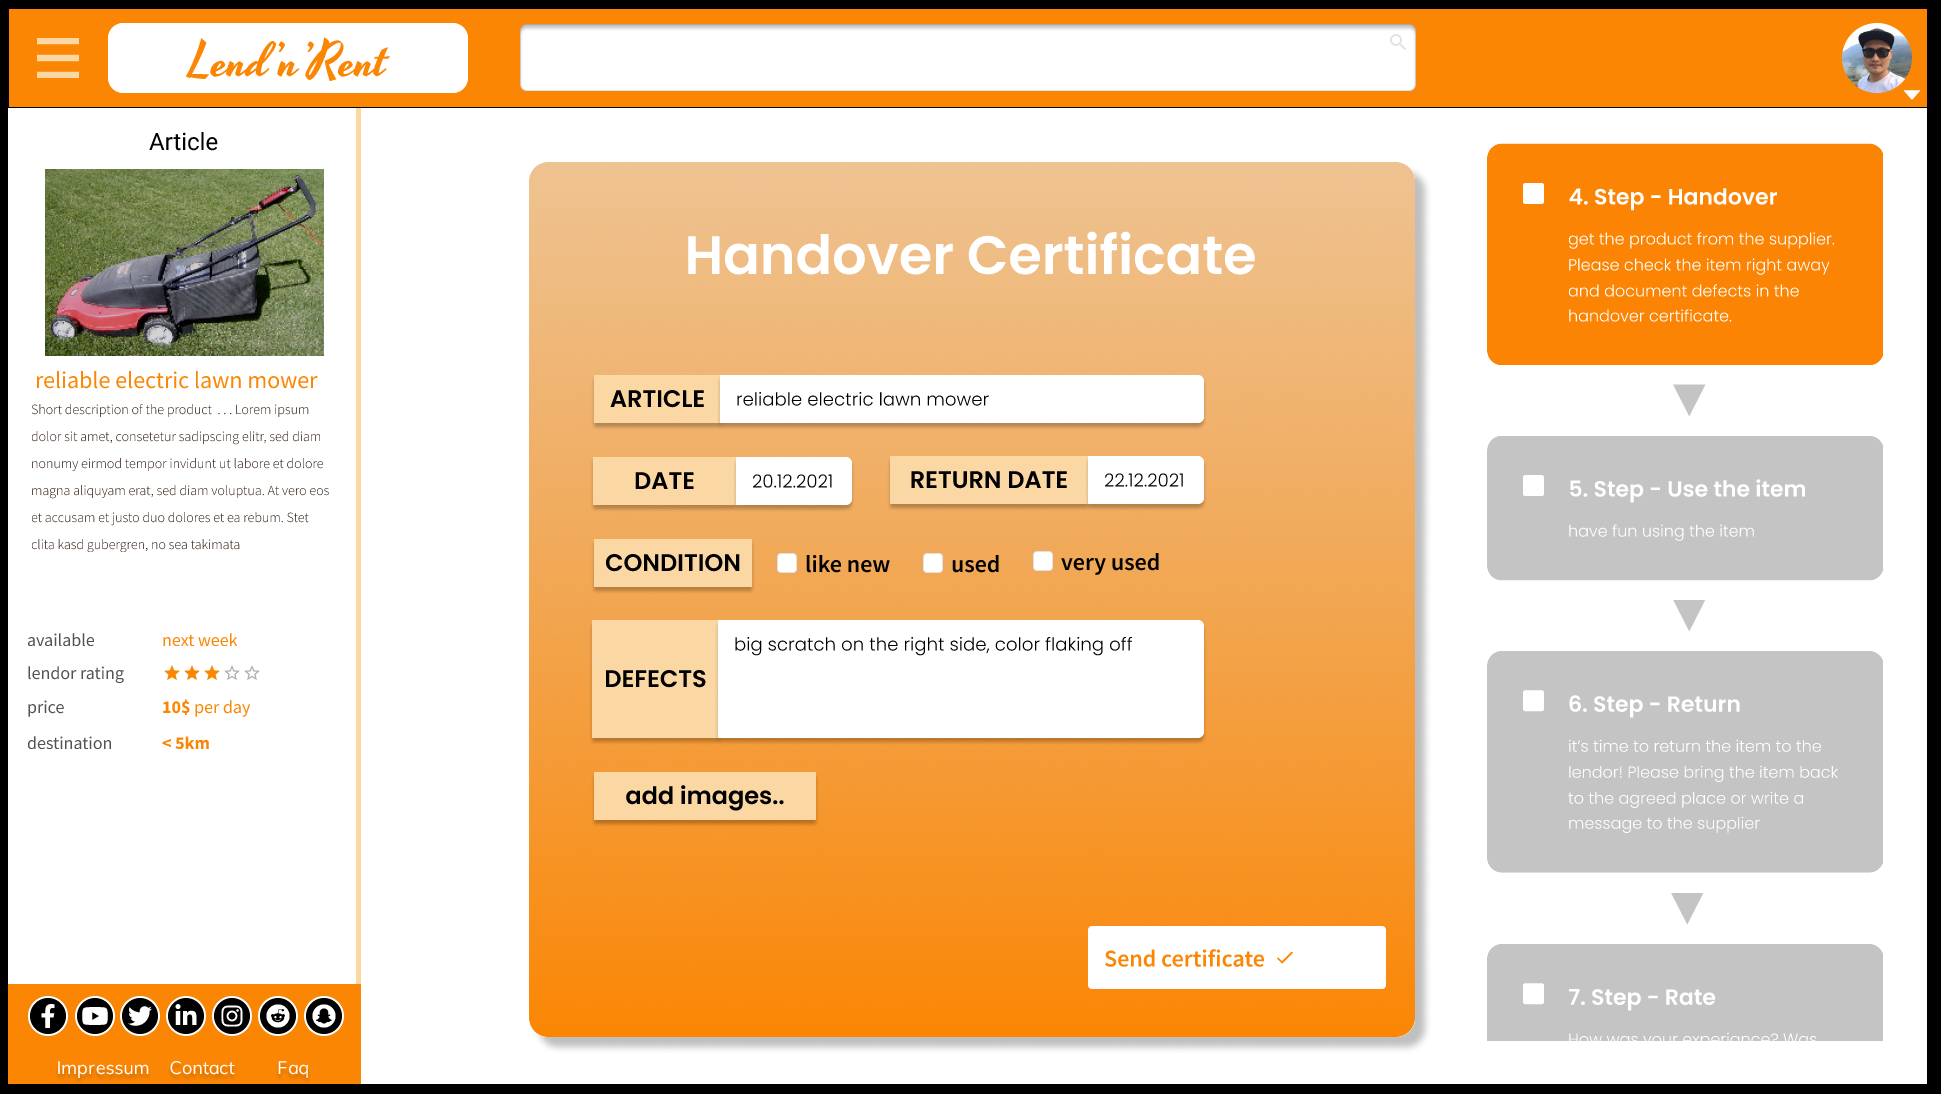
\includegraphics[width=0.49\linewidth]{abb/16step4con}
	\caption{Negotiation Step 4 Handover Certificate}
	\label{fig:Negotiation3}
	\centering
\end{figure}

\newpage
\noindent
After the transfer of the certificate, the renter can use the item. About the time of return both will be notified in time and have the opportunity to clarify the exact time in the chat.

\begin{figure}[H]
	\centering
	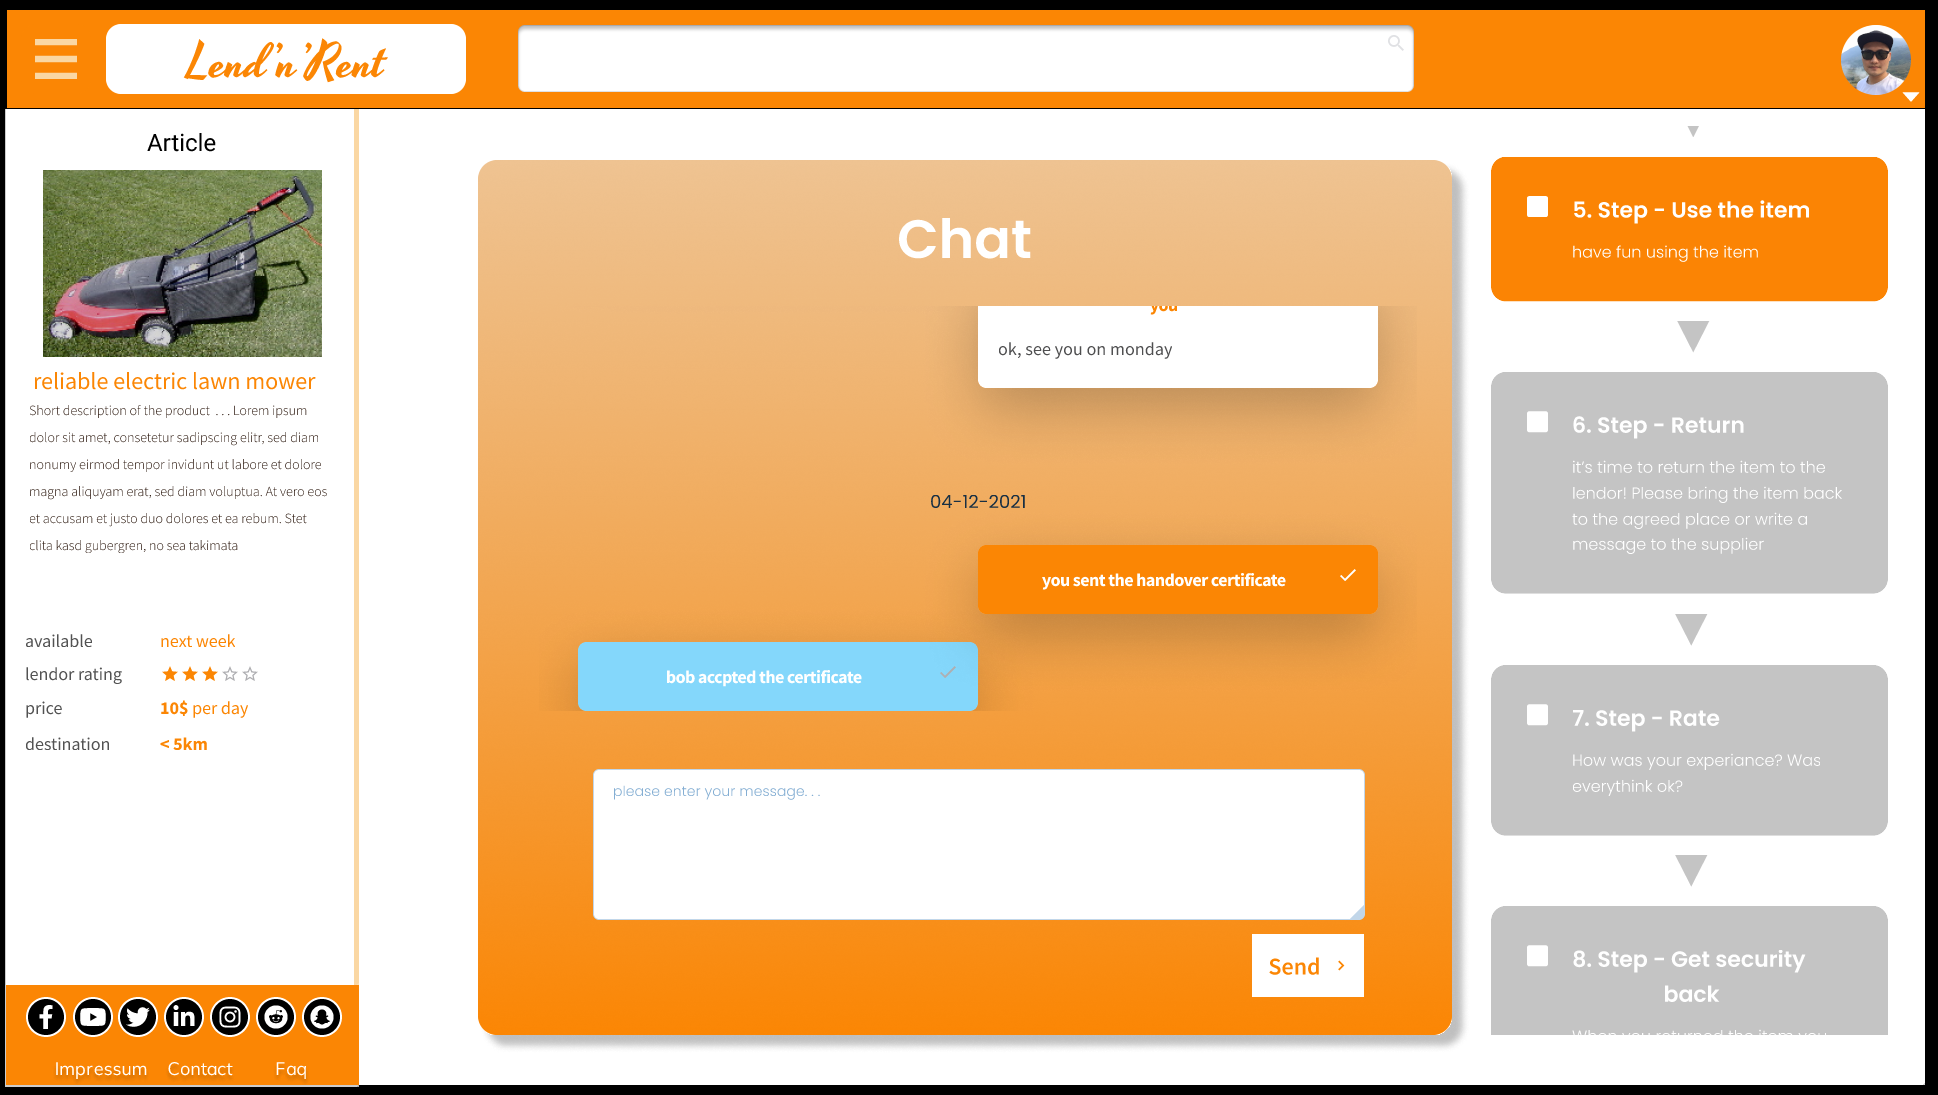
\includegraphics[width=0.49\linewidth]{abb/17step5}
	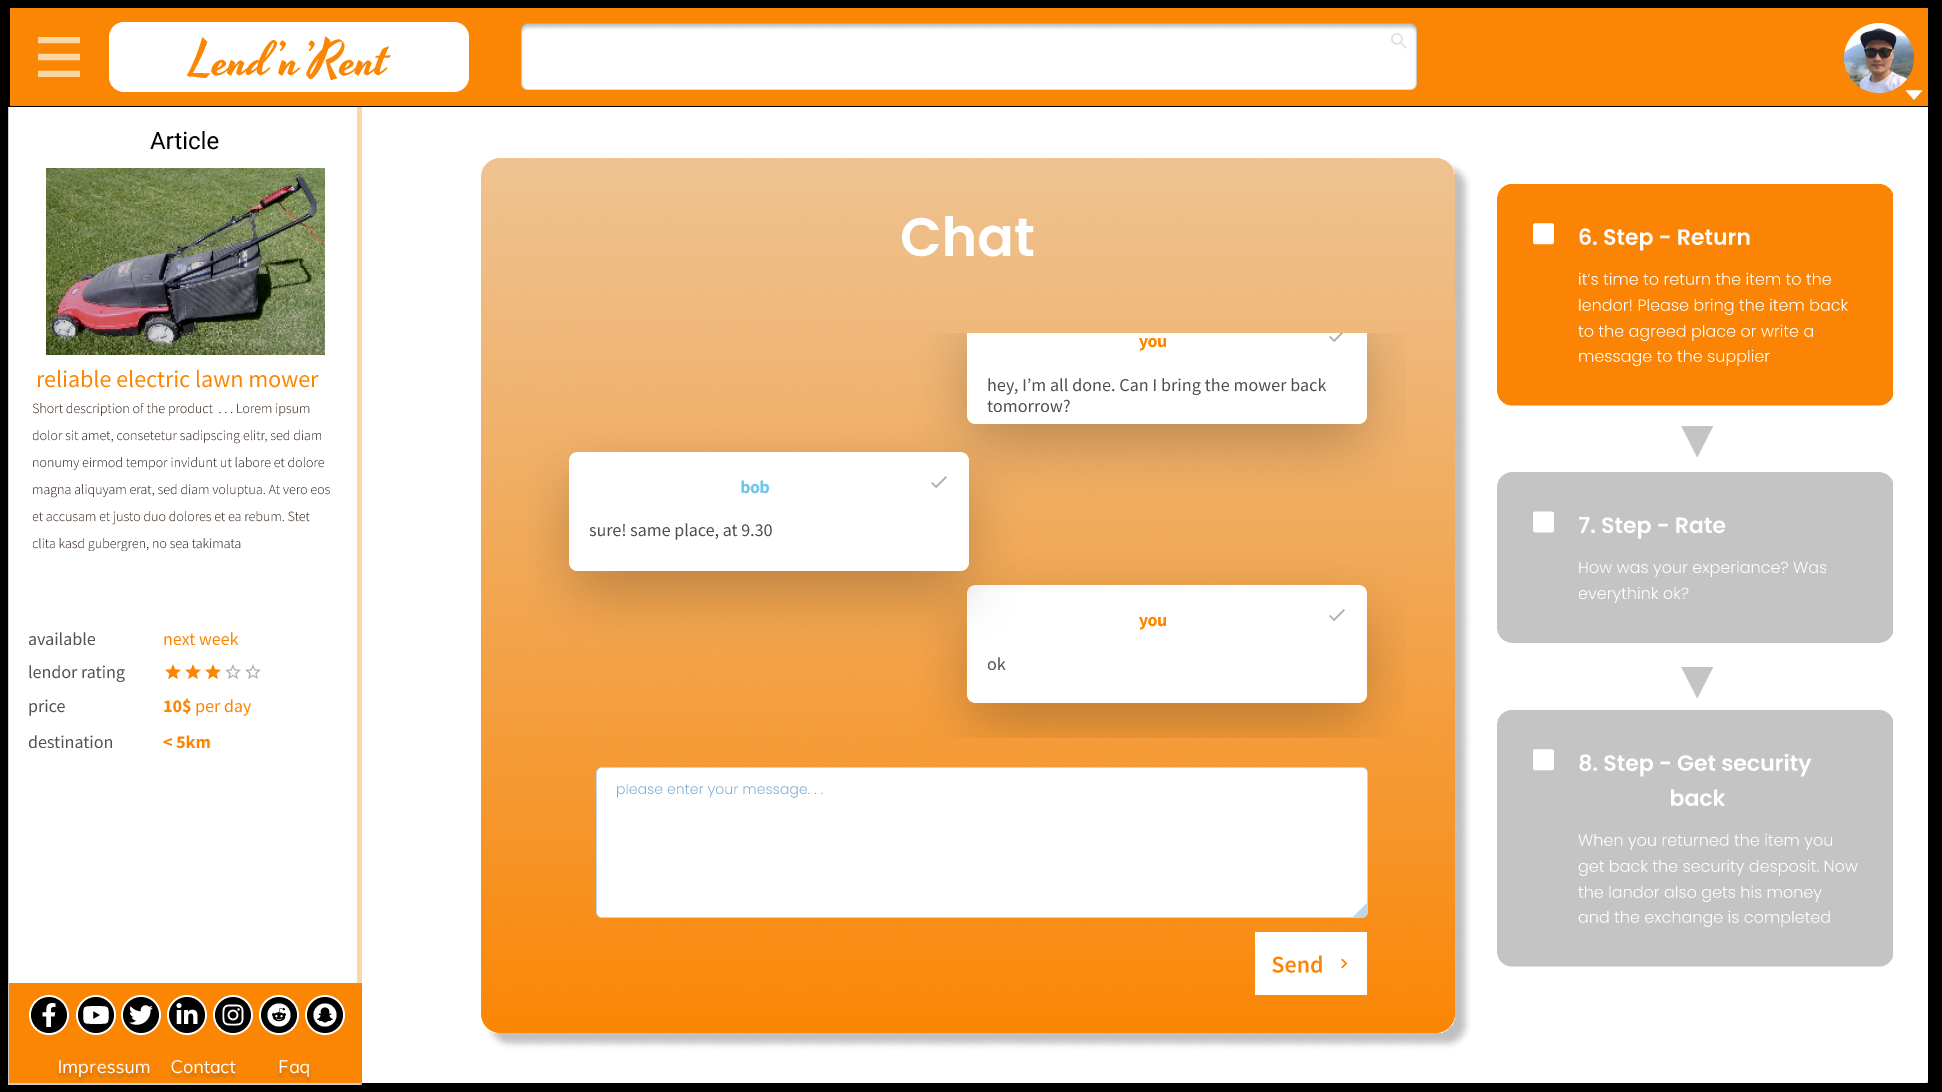
\includegraphics[width=0.49\linewidth]{abb/18step6}
	\caption{Use and Return}
	\label{fig:Negotiation4}
	\centering
\end{figure}

\noindent
After the return, the renter can rate the lender. if the item is returned in the same working condition, the renter gets back his security deposit and the lender gets the money.

\begin{figure}[H]
	\centering
	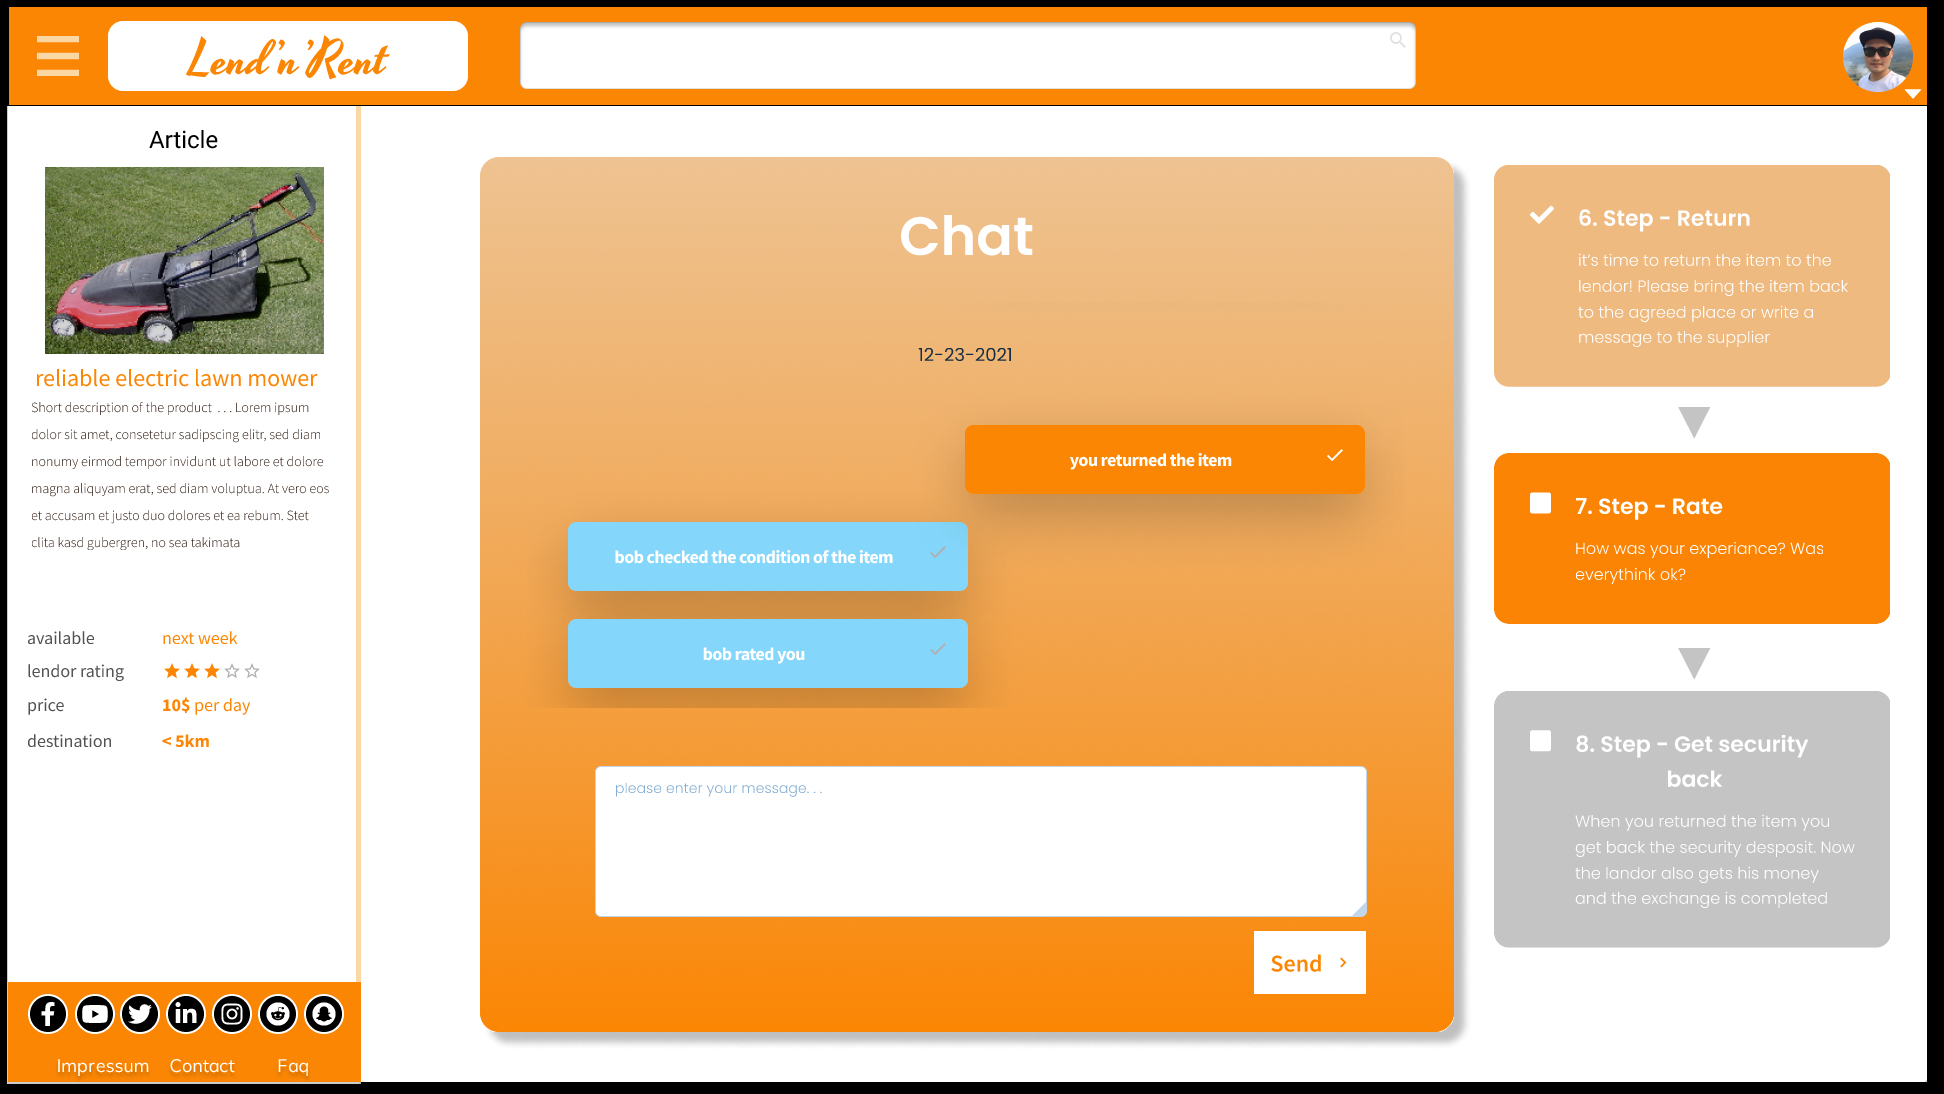
\includegraphics[width=0.49\linewidth]{abb/19step7}
	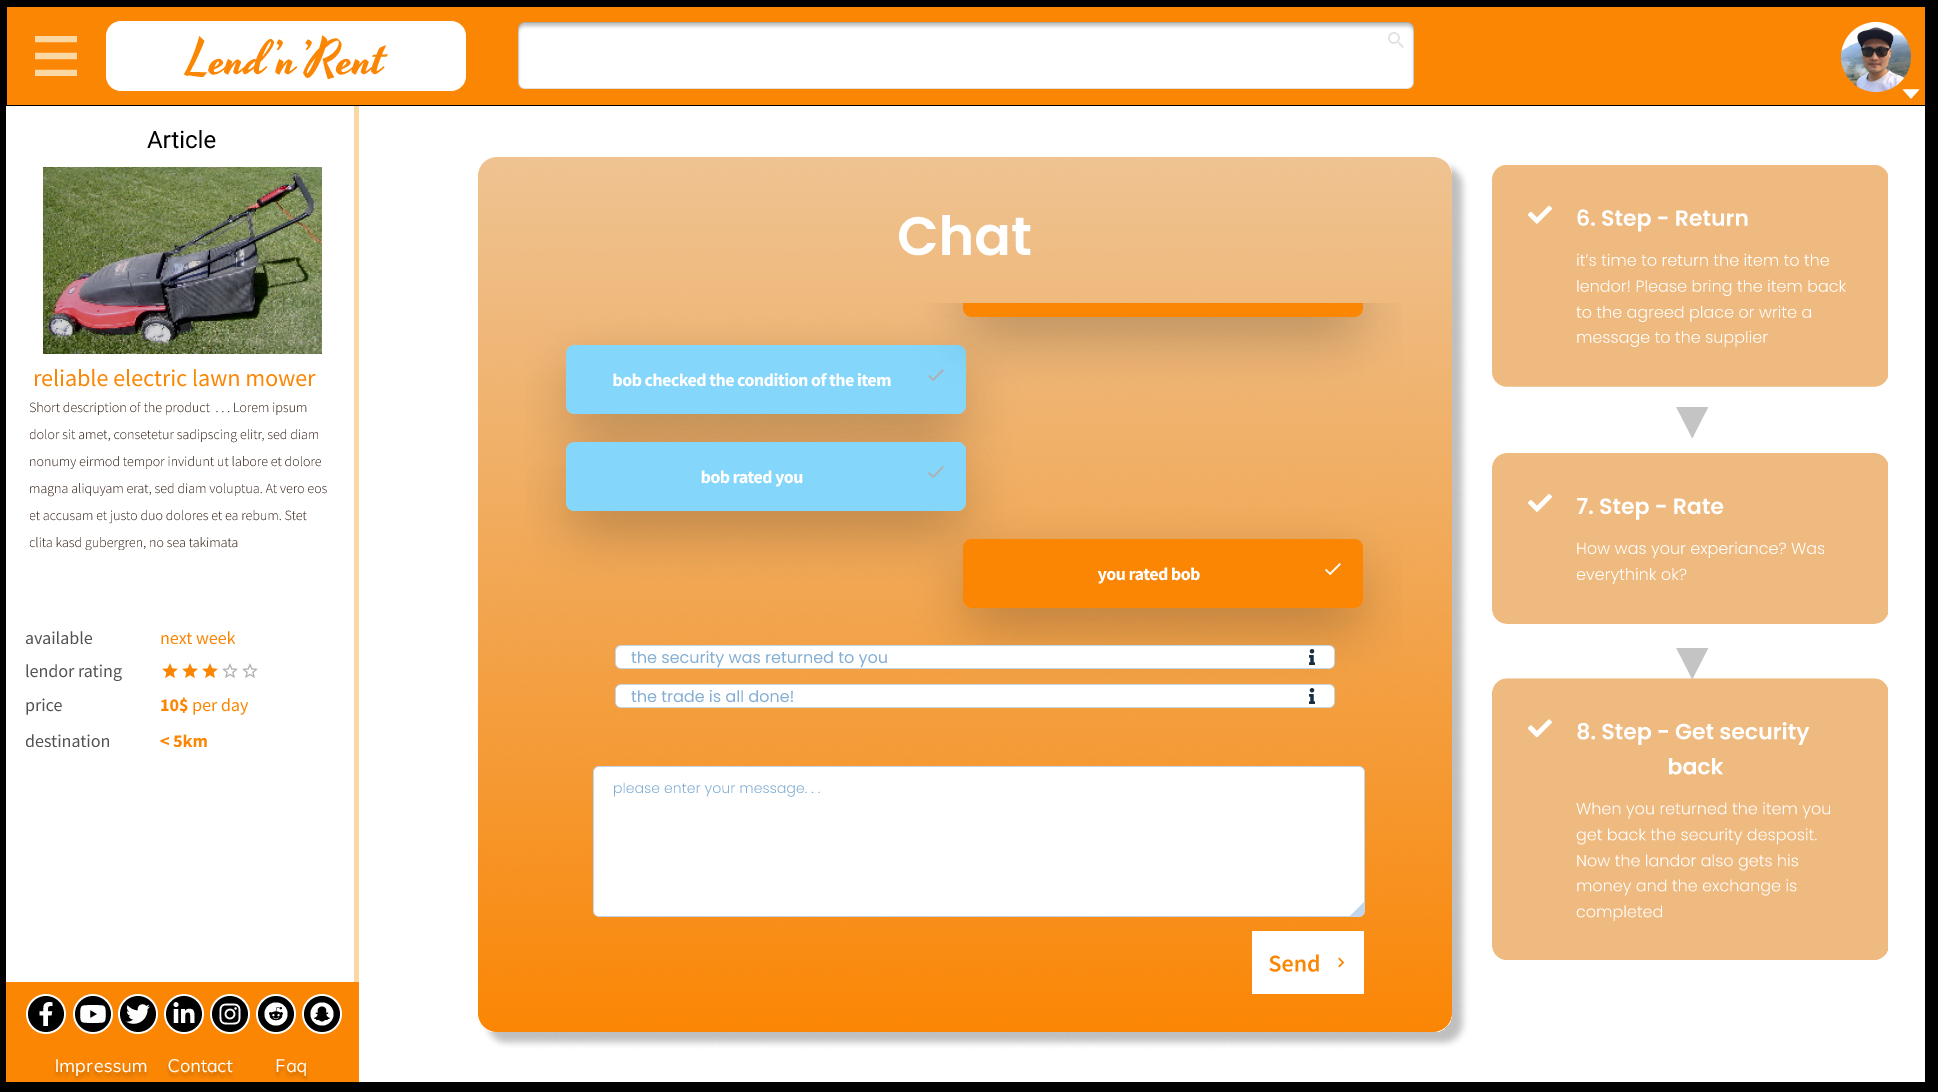
\includegraphics[width=0.49\linewidth]{abb/20steplast}
	\caption{Rating and Payment}
	\label{fig:Negotiation5}
	\centering
\end{figure}

\noindent
The design of the message page is adapted to the page design. In this way, the user can always distinguish whether he is accessing the messages with requests or those where he wants to rent something himself.

\begin{figure}[H]
	\centering
	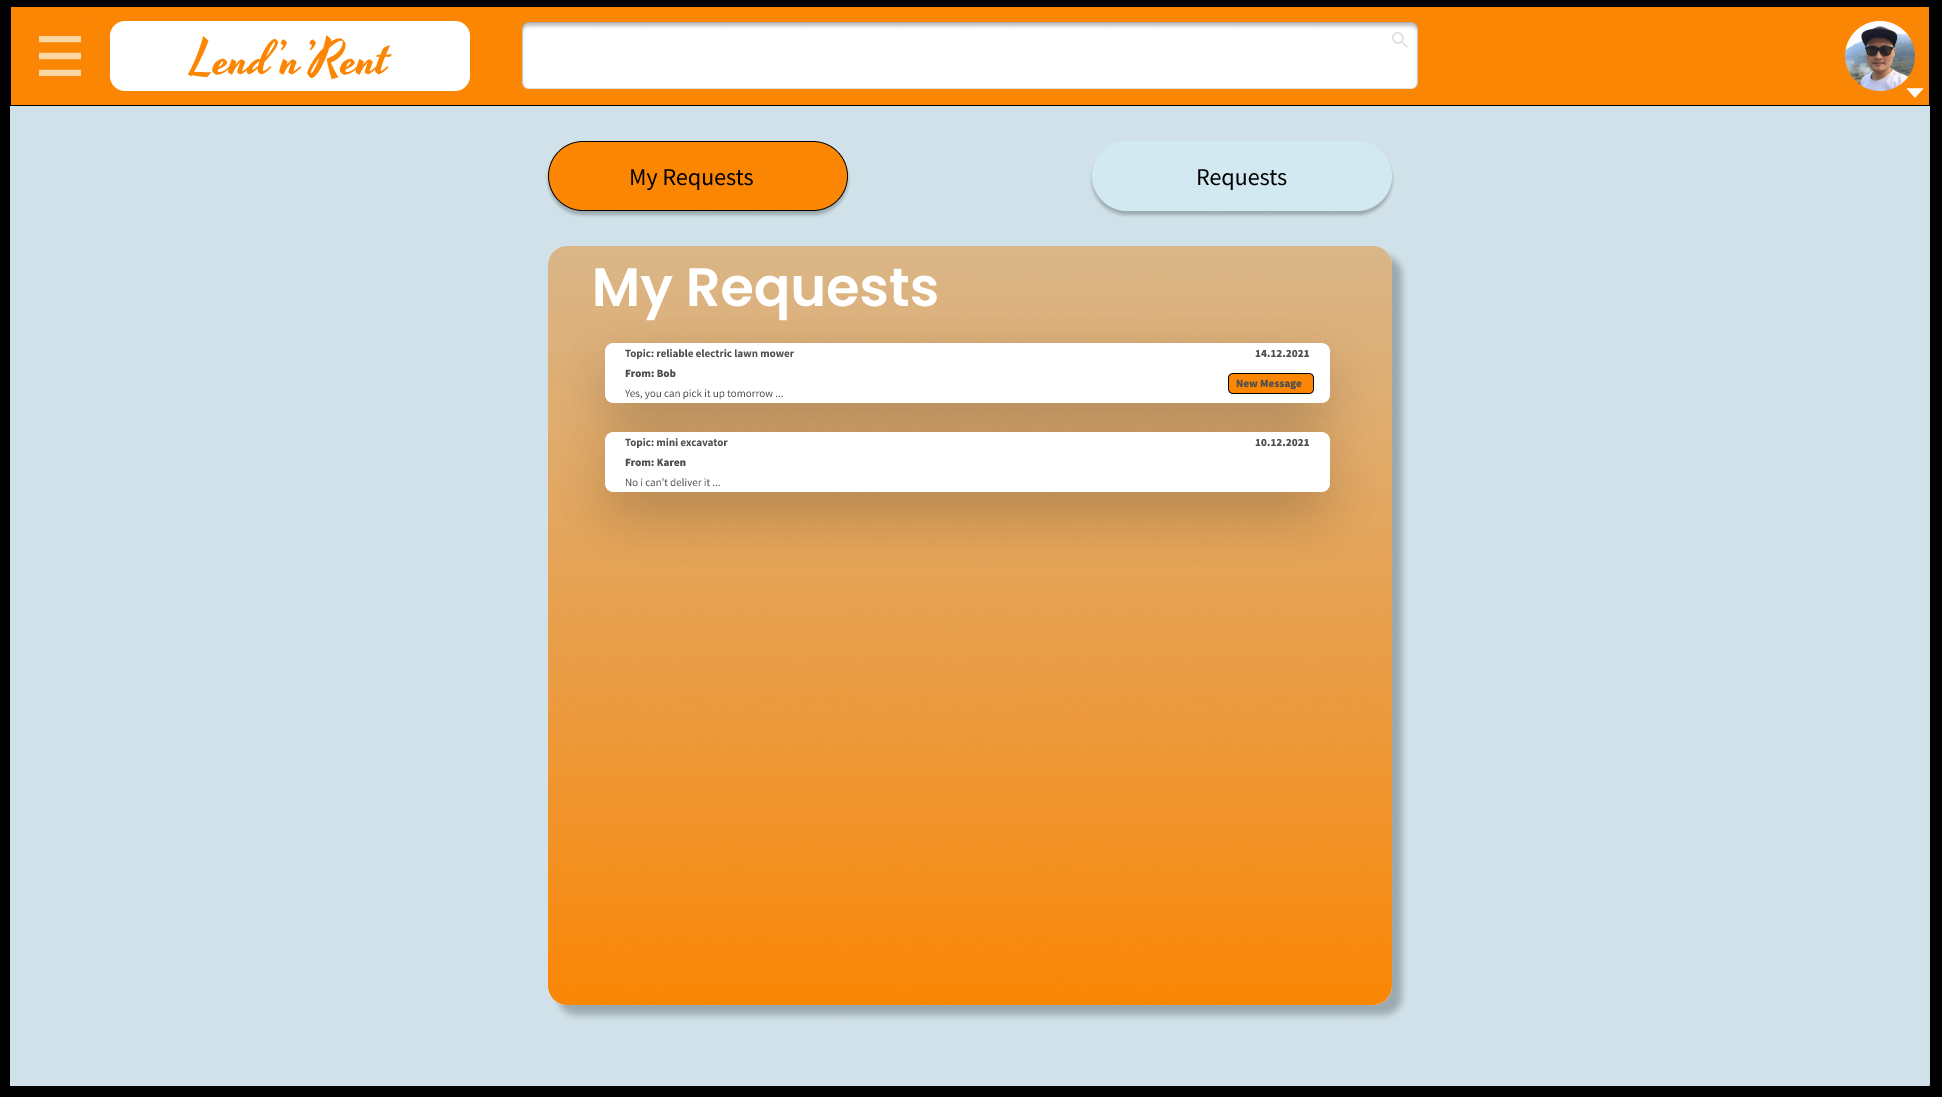
\includegraphics[width=0.49\linewidth]{abb/22chatrent}
	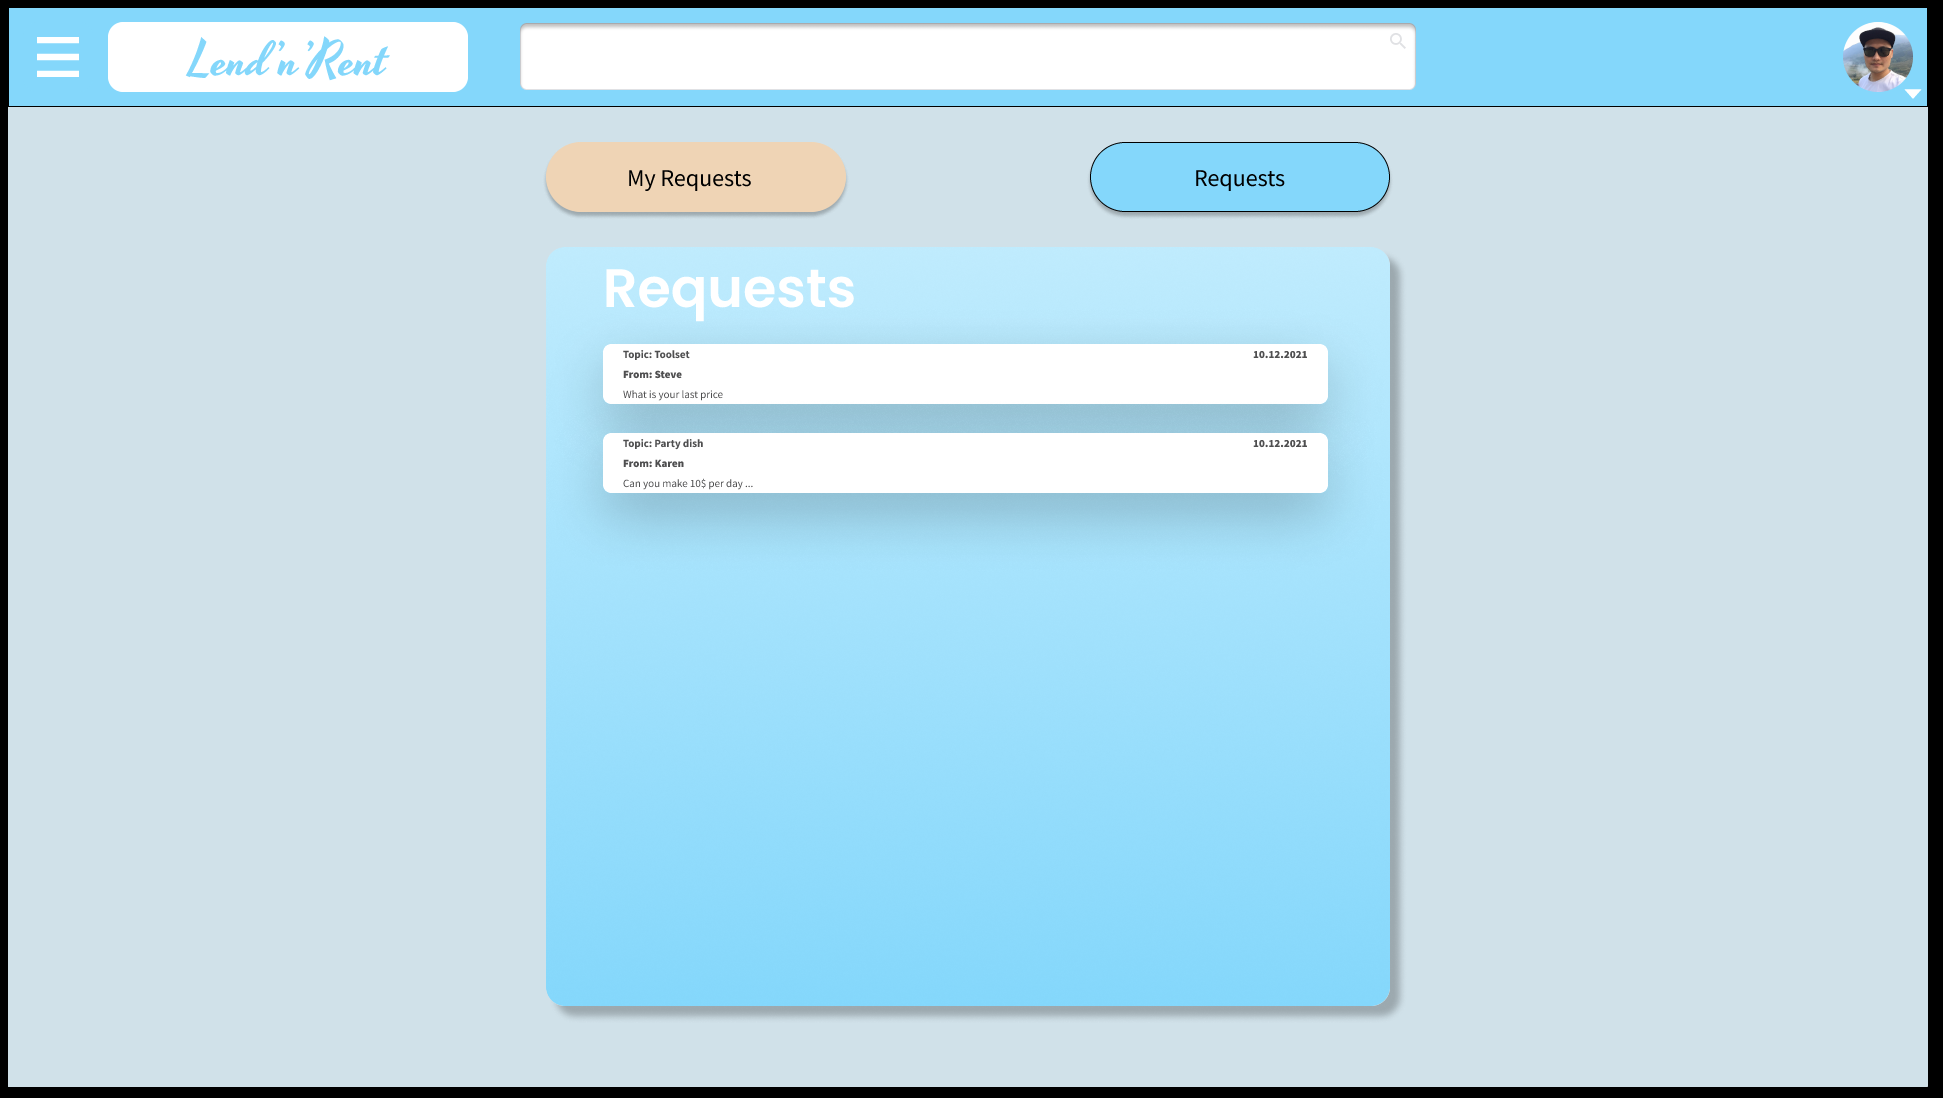
\includegraphics[width=0.49\linewidth]{abb/21chatlend}
	\caption{Messege view of lender and renter}
	\label{fig:messages}
	\centering
\end{figure}